% !TeX root = main.tex
% **************************************************************************************************************
% A Classic Thesis Style
% An Homage to The Elements of Typographic Style
%
% Copyright (C) 2018 André Miede and Ivo Pletikosić
%
% If you like the style then I would appreciate a postcard. My address
% can be found in the file ClassicThesis.pdf. A collection of the
% postcards I received so far is available online at
% http://postcards.miede.de
%
% License:
% This program is free software; you can redistribute it and/or modify
% it under the terms of the GNU General Public License as published by
% the Free Software Foundation; either version 2 of the License, or
% (at your option) any later version.
%
% This program is distributed in the hope that it will be useful,
% but WITHOUT ANY WARRANTY; without even the implied warranty of
% MERCHANTABILITY or FITNESS FOR A PARTICULAR PURPOSE.  See the
% GNU General Public License for more details.
%
% You should have received a copy of the GNU General Public License
% along with this program; see the file COPYING.  If not, write to
% the Free Software Foundation, Inc., 59 Temple Place - Suite 330,
% Boston, MA 02111-1307, USA.
%
% PLEASE SEE ALSO THE AUTHORS' NOTE REGARDING THIS LICENSE
% IN THE DOCUMENTATION (ClassicThesis.pdf --> Chapter 1 / Chapter01.tex)
% **************************************************************************************************************
\DocumentMetadata{} % to load the PDF management tools - Needed for newpax


\RequirePackage{silence} % :-\
    \WarningFilter{scrreprt}{Usage of package `titlesec'}
    %\WarningFilter{scrreprt}{Activating an ugly workaround}
    \WarningFilter{titlesec}{Non standard sectioning command detected}
\documentclass[ twoside,openright,titlepage,numbers=noenddot,%1headlines,
                headinclude,footinclude,cleardoublepage=empty,abstract=on,
                BCOR=5mm,paper=a4,fontsize=11pt]{scrreprt}

%********************************************************************
% Note: Make all your adjustments in here
%*******************************************************
% ****************************************************************************************************
% classicthesis-config.tex
% formerly known as loadpackages.sty, classicthesis-ldpkg.sty, and classicthesis-preamble.sty
% Use it at the beginning of your ClassicThesis.tex, or as a LaTeX Preamble
% in your ClassicThesis.{tex,lyx} with % ****************************************************************************************************
% classicthesis-config.tex
% formerly known as loadpackages.sty, classicthesis-ldpkg.sty, and classicthesis-preamble.sty
% Use it at the beginning of your ClassicThesis.tex, or as a LaTeX Preamble
% in your ClassicThesis.{tex,lyx} with % ****************************************************************************************************
% classicthesis-config.tex
% formerly known as loadpackages.sty, classicthesis-ldpkg.sty, and classicthesis-preamble.sty
% Use it at the beginning of your ClassicThesis.tex, or as a LaTeX Preamble
% in your ClassicThesis.{tex,lyx} with \input{classicthesis-config}
% ****************************************************************************************************
% If you like the classicthesis, then I would appreciate a postcard.
% My address can be found in the file ClassicThesis.pdf. A collection
% of the postcards I received so far is available online at
% http://postcards.miede.de
% ****************************************************************************************************


% ****************************************************************************************************
% 0. Set the encoding of your files. UTF-8 is the only sensible encoding nowadays. If you can't read
% äöüßáéçèê∂åëæƒÏ€ then change the encoding setting in your editor, not the line below. If your editor
% does not support utf8 use another editor!
% ****************************************************************************************************
%\PassOptionsToPackage{utf8}{inputenc}
%  \usepackage{inputenc}

%\PassOptionsToPackage{T1}{fontenc} % T2A for cyrillics
%  \usepackage{fontenc}
\PassOptionsToPackage{no-math}{fontspec}
	\usepackage{fontspec}

\usepackage{microtype}
\usepackage{selnolig}

% ****************************************************************************************************
% 1. Configure classicthesis for your needs here, e.g., remove "drafting" below
% in order to deactivate the time-stamp on the pages
% (see ClassicThesis.pdf for more information):
% ****************************************************************************************************
\PassOptionsToPackage{
  drafting=false,    % print version information on the bottom of the pages
  tocaligned=false, % the left column of the toc will be aligned (no indentation)
  dottedtoc=false,  % page numbers in ToC flushed right
  eulerchapternumbers=true, % use AMS Euler for chapter font (otherwise Palatino)
  linedheaders=false,       % chaper headers will have line above and beneath
  floatperchapter=true,     % numbering per chapter for all floats (i.e., Figure 1.1)
  eulermath=false,  % use awesome Euler fonts for mathematical formulae (only with pdfLaTeX)
  beramono=true,    % toggle a nice monospaced font (w/ bold)
  palatino=false,    % deactivate standard font for loading another one, see the last section at the end of this file for suggestions
  style=classicthesis % classicthesis, arsclassica
}{classicthesis}


% ****************************************************************************************************
% 2. Personal data and user ad-hoc commands (insert your own data here)
% ****************************************************************************************************
\newcommand{\myTitle}{
Quantum Dynamics of Disordered Many-body Spin Systems\xspace}
\newcommand{\mySubtitle}{\xspace}
\newcommand{\myDegree}{Dr. rer. nat)\xspace}
\newcommand{\myName}{Adrian Lukas Braemer\xspace}
\newcommand{\myProf}{Put name here\xspace}
\newcommand{\myOtherProf}{Put name here\xspace}
\newcommand{\mySupervisor}{Put name here\xspace}
\newcommand{\myFaculty}{Put data here\xspace}
\newcommand{\myDepartment}{Put data here\xspace}
\newcommand{\myUni}{Put data here\xspace}
\newcommand{\myLocation}{Heidelberg\xspace}
\newcommand{\myTime}{November 2024\xspace}
\newcommand{\myVersion}{\classicthesis}

% ********************************************************************
% Setup, finetuning, and useful commands
% ********************************************************************
\providecommand{\mLyX}{L\kern-.1667em\lower.25em\hbox{Y}\kern-.125emX\@}
\newcommand{\ie}{i.\,e.}
\newcommand{\Ie}{I.\,e.}
\newcommand{\eg}{e.\,g.}
\newcommand{\Eg}{E.\,g.}
% ****************************************************************************************************


% ****************************************************************************************************
% 3. Loading some handy packages
% ****************************************************************************************************
% ********************************************************************
% Packages with options that might require adjustments
% ********************************************************************
\PassOptionsToPackage{ngerman,american}{babel} % change this to your language(s), main language last
    \usepackage{babel}
%\usepackage{polyglossia}
%\setdefaultlanguage{english}
%\setotherlanguage{german}

\usepackage{csquotes}
% \PassOptionsToPackage{%
%   %backend=biber,bibencoding=utf8, %instead of bibtex
%   backend=bibtex8,bibencoding=ascii,%
%   language=auto,%
%   style=numeric-comp,%
%   url=false,
%   defernumbers=true,
%   %style=authoryear-comp, % Author 1999, 2010
%   %bibstyle=authoryear,dashed=false, % dashed: substitute rep. author with ---
%   % sorting=ynt, % name, year, title
%   sorting=none, % none
%   maxbibnames=10, % default: 3, et al.
%   %backref=true,%
%   natbib=true % natbib compatibility mode (\citep and \citet still work)
% }{biblatex}
%     \usepackage{biblatex}
\PassOptionsToPackage{%
  backend=biber,bibencoding=utf8, %instead of bibtex
  %backend=bibtex8,bibencoding=ascii,%
  defernumbers=true,
  language=auto,%
  %style=numeric-comp,%
  %style=authoryear-comp, % Author 1999, 2010
  style=phys,biblabel=brackets,%dashed=false, % dashed: substitute rep. author with ---
  sorting=none, % name, year, title
  maxbibnames=15, % default: 3, et al.
  %backref=true,%
  natbib=true % natbib compatibility mode (\citep and \citet still work)
}{biblatex}
    \usepackage{biblatex}


%\PassOptionsToPackage{fleqn}{amsmath}       % math environments and more by the AMS
%  \usepackage{amsmath}

% ********************************************************************
% General useful packages
% ********************************************************************
\usepackage{graphicx} %
\graphicspath{{gfx}}
\usepackage{scrhack} % fix warnings when using KOMA with listings package
\usepackage{xspace} % to get the spacing after macros right
\PassOptionsToPackage{printonlyused,smaller}{acronym}
  \usepackage{acronym} % nice macros for handling all acronyms in the thesis
  %\renewcommand{\bflabel}[1]{{#1}\hfill} % fix the list of acronyms --> no longer working
  %\renewcommand*{\acsfont}[1]{\textsc{#1}}
  %\renewcommand*{\aclabelfont}[1]{\acsfont{#1}}
  %\def\bflabel#1{{#1\hfill}}
  \def\bflabel#1{{\acsfont{#1}\hfill}}
  \def\aclabelfont#1{\acsfont{#1}}
% ****************************************************************************************************
%\usepackage{pgfplots} % External TikZ/PGF support (thanks to Andreas Nautsch)
%\usetikzlibrary{external}
%\tikzexternalize[mode=list and make, prefix=ext-tikz/]
% ****************************************************************************************************


% ****************************************************************************************************
% 4. Setup floats: tables, (sub)figures, and captions
% ****************************************************************************************************
\usepackage{tabularx} % better tables
  \setlength{\extrarowheight}{3pt} % increase table row height
\newcommand{\tableheadline}[1]{\multicolumn{1}{l}{\spacedlowsmallcaps{#1}}}
\newcommand{\myfloatalign}{\centering} % to be used with each float for alignment
\usepackage{subfig}
% ****************************************************************************************************


% ****************************************************************************************************
% 5. Setup code listings
% ****************************************************************************************************
\usepackage{listings}
%\lstset{emph={trueIndex,root},emphstyle=\color{BlueViolet}}%\underbar} % for special keywords
\lstset{language=[LaTeX]Tex,%C++,
  morekeywords={PassOptionsToPackage,selectlanguage},
  keywordstyle=\color{RoyalBlue},%\bfseries,
  basicstyle=\small\ttfamily,
  %identifierstyle=\color{NavyBlue},
  commentstyle=\color{Green}\ttfamily,
  stringstyle=\rmfamily,
  numbers=none,%left,%
  numberstyle=\scriptsize,%\tiny
  stepnumber=5,
  numbersep=8pt,
  showstringspaces=false,
  breaklines=true,
  %frameround=ftff,
  %frame=single,
  belowcaptionskip=.75\baselineskip
  %frame=L
}
% ****************************************************************************************************




% ****************************************************************************************************
% 6. Last calls before the bar closes
% ****************************************************************************************************
\usepackage{ragged2e}

\usepackage{mathtools,amsfonts,amsthm, amssymb,bm}
\DeclarePairedDelimiter\norm{\lVert}{\rVert}

%\usepackage{braket}
\usepackage{physics2}
\usephysicsmodule{braket}

%\usepackage{mathrsfs} % \mathscr
\usepackage{dsfont} % double stroke \mathds

\DeclareMathOperator{\Tr}{Tr}
\usepackage{afterpage}
\usepackage{algorithm}
\usepackage[noend]{algpseudocode}


% ********************************************************************
% Her Majesty herself
% ********************************************************************
\usepackage{classicthesis}

% Palatino fonts - these packages have better spacing than the ones used by classicthesis so load them separately
%\usepackage[theoremfont,trueslanted,largesc,p,osf]{newpxtext}
%\usepackage[fracspacing,varbb]{newpxmath}
%\linespread{1.05} % a bit more for Palatino

% ********************************************************************
% Fine-tune hyperreferences (hyperref should be called last)
% ********************************************************************
\hypersetup{%
  %draft, % hyperref's draft mode, for printing see below
  %colorlinks=true, linktocpage=true, pdfstartpage=3, pdfstartview=FitV,%
  % uncomment the following line if you want to have black links (e.g., for printing)
  colorlinks=false, linktocpage=false, pdfstartpage=3, pdfstartview=FitV, pdfborder={0 0 0},%
  breaklinks=true, pageanchor=true,%
  pdfpagemode=UseNone, %
  % pdfpagemode=UseOutlines,%
  plainpages=false, bookmarksnumbered, bookmarksopen=true, bookmarksopenlevel=1,%
  hypertexnames=true, pdfhighlight=/O,%nesting=true,%frenchlinks,%
  urlcolor=CTurl, linkcolor=CTlink, citecolor=CTcitation, %pagecolor=RoyalBlue,%
  %urlcolor=Black, linkcolor=Black, citecolor=Black, %pagecolor=Black,%
  pdftitle={\myTitle},%
  pdfauthor={\textcopyright\ \myName, \myUni, \myFaculty},%
  pdfsubject={},%
  pdfkeywords={},%
  pdfcreator={luaLaTeX},%
  pdfproducer={LaTeX with hyperref and classicthesis}%
}


% ********************************************************************
% Setup autoreferences (hyperref and babel)
% ********************************************************************
% There are some issues regarding autorefnames
% http://www.tex.ac.uk/cgi-bin/texfaq2html?label=latexwords
% you have to redefine the macros for the
% language you use, e.g., american, ngerman
% (as chosen when loading babel/AtBeginDocument)
% ********************************************************************
\makeatletter
\@ifpackageloaded{babel}%
  {%
    \addto\extrasamerican{%
      \renewcommand*{\figureautorefname}{Figure}%
      \renewcommand*{\tableautorefname}{Table}%
      \renewcommand*{\partautorefname}{Part}%
      \renewcommand*{\chapterautorefname}{Chapter}%
      \renewcommand*{\sectionautorefname}{Section}%
      \renewcommand*{\subsectionautorefname}{Section}%
      \renewcommand*{\subsubsectionautorefname}{Section}%
    }%
    \addto\extrasngerman{%
      \renewcommand*{\paragraphautorefname}{Absatz}%
      \renewcommand*{\subparagraphautorefname}{Unterabsatz}%
      \renewcommand*{\footnoteautorefname}{Fu\"snote}%
      \renewcommand*{\FancyVerbLineautorefname}{Zeile}%
      \renewcommand*{\theoremautorefname}{Theorem}%
      \renewcommand*{\appendixautorefname}{Anhang}%
      \renewcommand*{\equationautorefname}{Gleichung}%
      \renewcommand*{\itemautorefname}{Punkt}%
    }%
      % Fix to getting autorefs for subfigures right (thanks to Belinda Vogt for changing the definition)
      \providecommand{\subfigureautorefname}{\figureautorefname}%
    }{\relax}
\makeatother


% ********************************************************************
% Development Stuff
% ********************************************************************
\listfiles
%\PassOptionsToPackage{l2tabu,orthodox,abort}{nag}
%  \usepackage{nag}
%\PassOptionsToPackage{warning, all}{onlyamsmath}
%  \usepackage{onlyamsmath}


% ****************************************************************************************************
% 7. Further adjustments (experimental)
% ****************************************************************************************************
% ********************************************************************
% Changing the text area
% ********************************************************************
%\areaset[current]{312pt}{761pt} % 686 (factor 2.2) + 33 head + 42 head \the\footskip
%\setlength{\marginparwidth}{7em}%
%\setlength{\marginparsep}{2em}%

% ********************************************************************
% Using different fonts
% ********************************************************************
%\usepackage[oldstylenums]{kpfonts} % oldstyle notextcomp
% \usepackage[osf]{libertine}
%\usepackage[light,condensed,math]{iwona}
%\renewcommand{\sfdefault}{iwona}
%\usepackage{lmodern} % <-- no osf support :-(
%\usepackage{cfr-lm} %
%\usepackage[urw-garamond]{mathdesign} <-- no osf support :-(
%\usepackage[default,osfigures]{opensans} % scale=0.95
%\usepackage[sfdefault]{FiraSans}
% \usepackage[opticals,mathlf]{MinionPro} % onlytext
% ********************************************************************
%\usepackage[largesc,osf]{newpxtext}
%\linespread{1.05} % a bit more for Palatino
% Used to fix these:
% https://bitbucket.org/amiede/classicthesis/issues/139/italics-in-pallatino-capitals-chapter
% https://bitbucket.org/amiede/classicthesis/issues/45/problema-testatine-su-classicthesis-style
% ********************************************************************
% ****************************************************************************************************

% ****************************************************************************************************
% If you like the classicthesis, then I would appreciate a postcard.
% My address can be found in the file ClassicThesis.pdf. A collection
% of the postcards I received so far is available online at
% http://postcards.miede.de
% ****************************************************************************************************


% ****************************************************************************************************
% 0. Set the encoding of your files. UTF-8 is the only sensible encoding nowadays. If you can't read
% äöüßáéçèê∂åëæƒÏ€ then change the encoding setting in your editor, not the line below. If your editor
% does not support utf8 use another editor!
% ****************************************************************************************************
%\PassOptionsToPackage{utf8}{inputenc}
%  \usepackage{inputenc}

%\PassOptionsToPackage{T1}{fontenc} % T2A for cyrillics
%  \usepackage{fontenc}
\PassOptionsToPackage{no-math}{fontspec}
	\usepackage{fontspec}

\usepackage{microtype}
\usepackage{selnolig}

% ****************************************************************************************************
% 1. Configure classicthesis for your needs here, e.g., remove "drafting" below
% in order to deactivate the time-stamp on the pages
% (see ClassicThesis.pdf for more information):
% ****************************************************************************************************
\PassOptionsToPackage{
  drafting=false,    % print version information on the bottom of the pages
  tocaligned=false, % the left column of the toc will be aligned (no indentation)
  dottedtoc=false,  % page numbers in ToC flushed right
  eulerchapternumbers=true, % use AMS Euler for chapter font (otherwise Palatino)
  linedheaders=false,       % chaper headers will have line above and beneath
  floatperchapter=true,     % numbering per chapter for all floats (i.e., Figure 1.1)
  eulermath=false,  % use awesome Euler fonts for mathematical formulae (only with pdfLaTeX)
  beramono=true,    % toggle a nice monospaced font (w/ bold)
  palatino=false,    % deactivate standard font for loading another one, see the last section at the end of this file for suggestions
  style=classicthesis % classicthesis, arsclassica
}{classicthesis}


% ****************************************************************************************************
% 2. Personal data and user ad-hoc commands (insert your own data here)
% ****************************************************************************************************
\newcommand{\myTitle}{
Quantum Dynamics of Disordered Many-body Spin Systems\xspace}
\newcommand{\mySubtitle}{\xspace}
\newcommand{\myDegree}{Dr. rer. nat)\xspace}
\newcommand{\myName}{Adrian Lukas Braemer\xspace}
\newcommand{\myProf}{Put name here\xspace}
\newcommand{\myOtherProf}{Put name here\xspace}
\newcommand{\mySupervisor}{Put name here\xspace}
\newcommand{\myFaculty}{Put data here\xspace}
\newcommand{\myDepartment}{Put data here\xspace}
\newcommand{\myUni}{Put data here\xspace}
\newcommand{\myLocation}{Heidelberg\xspace}
\newcommand{\myTime}{November 2024\xspace}
\newcommand{\myVersion}{\classicthesis}

% ********************************************************************
% Setup, finetuning, and useful commands
% ********************************************************************
\providecommand{\mLyX}{L\kern-.1667em\lower.25em\hbox{Y}\kern-.125emX\@}
\newcommand{\ie}{i.\,e.}
\newcommand{\Ie}{I.\,e.}
\newcommand{\eg}{e.\,g.}
\newcommand{\Eg}{E.\,g.}
% ****************************************************************************************************


% ****************************************************************************************************
% 3. Loading some handy packages
% ****************************************************************************************************
% ********************************************************************
% Packages with options that might require adjustments
% ********************************************************************
\PassOptionsToPackage{ngerman,american}{babel} % change this to your language(s), main language last
    \usepackage{babel}
%\usepackage{polyglossia}
%\setdefaultlanguage{english}
%\setotherlanguage{german}

\usepackage{csquotes}
% \PassOptionsToPackage{%
%   %backend=biber,bibencoding=utf8, %instead of bibtex
%   backend=bibtex8,bibencoding=ascii,%
%   language=auto,%
%   style=numeric-comp,%
%   url=false,
%   defernumbers=true,
%   %style=authoryear-comp, % Author 1999, 2010
%   %bibstyle=authoryear,dashed=false, % dashed: substitute rep. author with ---
%   % sorting=ynt, % name, year, title
%   sorting=none, % none
%   maxbibnames=10, % default: 3, et al.
%   %backref=true,%
%   natbib=true % natbib compatibility mode (\citep and \citet still work)
% }{biblatex}
%     \usepackage{biblatex}
\PassOptionsToPackage{%
  backend=biber,bibencoding=utf8, %instead of bibtex
  %backend=bibtex8,bibencoding=ascii,%
  defernumbers=true,
  language=auto,%
  %style=numeric-comp,%
  %style=authoryear-comp, % Author 1999, 2010
  style=phys,biblabel=brackets,%dashed=false, % dashed: substitute rep. author with ---
  sorting=none, % name, year, title
  maxbibnames=15, % default: 3, et al.
  %backref=true,%
  natbib=true % natbib compatibility mode (\citep and \citet still work)
}{biblatex}
    \usepackage{biblatex}


%\PassOptionsToPackage{fleqn}{amsmath}       % math environments and more by the AMS
%  \usepackage{amsmath}

% ********************************************************************
% General useful packages
% ********************************************************************
\usepackage{graphicx} %
\graphicspath{{gfx}}
\usepackage{scrhack} % fix warnings when using KOMA with listings package
\usepackage{xspace} % to get the spacing after macros right
\PassOptionsToPackage{printonlyused,smaller}{acronym}
  \usepackage{acronym} % nice macros for handling all acronyms in the thesis
  %\renewcommand{\bflabel}[1]{{#1}\hfill} % fix the list of acronyms --> no longer working
  %\renewcommand*{\acsfont}[1]{\textsc{#1}}
  %\renewcommand*{\aclabelfont}[1]{\acsfont{#1}}
  %\def\bflabel#1{{#1\hfill}}
  \def\bflabel#1{{\acsfont{#1}\hfill}}
  \def\aclabelfont#1{\acsfont{#1}}
% ****************************************************************************************************
%\usepackage{pgfplots} % External TikZ/PGF support (thanks to Andreas Nautsch)
%\usetikzlibrary{external}
%\tikzexternalize[mode=list and make, prefix=ext-tikz/]
% ****************************************************************************************************


% ****************************************************************************************************
% 4. Setup floats: tables, (sub)figures, and captions
% ****************************************************************************************************
\usepackage{tabularx} % better tables
  \setlength{\extrarowheight}{3pt} % increase table row height
\newcommand{\tableheadline}[1]{\multicolumn{1}{l}{\spacedlowsmallcaps{#1}}}
\newcommand{\myfloatalign}{\centering} % to be used with each float for alignment
\usepackage{subfig}
% ****************************************************************************************************


% ****************************************************************************************************
% 5. Setup code listings
% ****************************************************************************************************
\usepackage{listings}
%\lstset{emph={trueIndex,root},emphstyle=\color{BlueViolet}}%\underbar} % for special keywords
\lstset{language=[LaTeX]Tex,%C++,
  morekeywords={PassOptionsToPackage,selectlanguage},
  keywordstyle=\color{RoyalBlue},%\bfseries,
  basicstyle=\small\ttfamily,
  %identifierstyle=\color{NavyBlue},
  commentstyle=\color{Green}\ttfamily,
  stringstyle=\rmfamily,
  numbers=none,%left,%
  numberstyle=\scriptsize,%\tiny
  stepnumber=5,
  numbersep=8pt,
  showstringspaces=false,
  breaklines=true,
  %frameround=ftff,
  %frame=single,
  belowcaptionskip=.75\baselineskip
  %frame=L
}
% ****************************************************************************************************




% ****************************************************************************************************
% 6. Last calls before the bar closes
% ****************************************************************************************************
\usepackage{ragged2e}

\usepackage{mathtools,amsfonts,amsthm, amssymb,bm}
\DeclarePairedDelimiter\norm{\lVert}{\rVert}

%\usepackage{braket}
\usepackage{physics2}
\usephysicsmodule{braket}

%\usepackage{mathrsfs} % \mathscr
\usepackage{dsfont} % double stroke \mathds

\DeclareMathOperator{\Tr}{Tr}
\usepackage{afterpage}
\usepackage{algorithm}
\usepackage[noend]{algpseudocode}


% ********************************************************************
% Her Majesty herself
% ********************************************************************
\usepackage{classicthesis}

% Palatino fonts - these packages have better spacing than the ones used by classicthesis so load them separately
%\usepackage[theoremfont,trueslanted,largesc,p,osf]{newpxtext}
%\usepackage[fracspacing,varbb]{newpxmath}
%\linespread{1.05} % a bit more for Palatino

% ********************************************************************
% Fine-tune hyperreferences (hyperref should be called last)
% ********************************************************************
\hypersetup{%
  %draft, % hyperref's draft mode, for printing see below
  %colorlinks=true, linktocpage=true, pdfstartpage=3, pdfstartview=FitV,%
  % uncomment the following line if you want to have black links (e.g., for printing)
  colorlinks=false, linktocpage=false, pdfstartpage=3, pdfstartview=FitV, pdfborder={0 0 0},%
  breaklinks=true, pageanchor=true,%
  pdfpagemode=UseNone, %
  % pdfpagemode=UseOutlines,%
  plainpages=false, bookmarksnumbered, bookmarksopen=true, bookmarksopenlevel=1,%
  hypertexnames=true, pdfhighlight=/O,%nesting=true,%frenchlinks,%
  urlcolor=CTurl, linkcolor=CTlink, citecolor=CTcitation, %pagecolor=RoyalBlue,%
  %urlcolor=Black, linkcolor=Black, citecolor=Black, %pagecolor=Black,%
  pdftitle={\myTitle},%
  pdfauthor={\textcopyright\ \myName, \myUni, \myFaculty},%
  pdfsubject={},%
  pdfkeywords={},%
  pdfcreator={luaLaTeX},%
  pdfproducer={LaTeX with hyperref and classicthesis}%
}


% ********************************************************************
% Setup autoreferences (hyperref and babel)
% ********************************************************************
% There are some issues regarding autorefnames
% http://www.tex.ac.uk/cgi-bin/texfaq2html?label=latexwords
% you have to redefine the macros for the
% language you use, e.g., american, ngerman
% (as chosen when loading babel/AtBeginDocument)
% ********************************************************************
\makeatletter
\@ifpackageloaded{babel}%
  {%
    \addto\extrasamerican{%
      \renewcommand*{\figureautorefname}{Figure}%
      \renewcommand*{\tableautorefname}{Table}%
      \renewcommand*{\partautorefname}{Part}%
      \renewcommand*{\chapterautorefname}{Chapter}%
      \renewcommand*{\sectionautorefname}{Section}%
      \renewcommand*{\subsectionautorefname}{Section}%
      \renewcommand*{\subsubsectionautorefname}{Section}%
    }%
    \addto\extrasngerman{%
      \renewcommand*{\paragraphautorefname}{Absatz}%
      \renewcommand*{\subparagraphautorefname}{Unterabsatz}%
      \renewcommand*{\footnoteautorefname}{Fu\"snote}%
      \renewcommand*{\FancyVerbLineautorefname}{Zeile}%
      \renewcommand*{\theoremautorefname}{Theorem}%
      \renewcommand*{\appendixautorefname}{Anhang}%
      \renewcommand*{\equationautorefname}{Gleichung}%
      \renewcommand*{\itemautorefname}{Punkt}%
    }%
      % Fix to getting autorefs for subfigures right (thanks to Belinda Vogt for changing the definition)
      \providecommand{\subfigureautorefname}{\figureautorefname}%
    }{\relax}
\makeatother


% ********************************************************************
% Development Stuff
% ********************************************************************
\listfiles
%\PassOptionsToPackage{l2tabu,orthodox,abort}{nag}
%  \usepackage{nag}
%\PassOptionsToPackage{warning, all}{onlyamsmath}
%  \usepackage{onlyamsmath}


% ****************************************************************************************************
% 7. Further adjustments (experimental)
% ****************************************************************************************************
% ********************************************************************
% Changing the text area
% ********************************************************************
%\areaset[current]{312pt}{761pt} % 686 (factor 2.2) + 33 head + 42 head \the\footskip
%\setlength{\marginparwidth}{7em}%
%\setlength{\marginparsep}{2em}%

% ********************************************************************
% Using different fonts
% ********************************************************************
%\usepackage[oldstylenums]{kpfonts} % oldstyle notextcomp
% \usepackage[osf]{libertine}
%\usepackage[light,condensed,math]{iwona}
%\renewcommand{\sfdefault}{iwona}
%\usepackage{lmodern} % <-- no osf support :-(
%\usepackage{cfr-lm} %
%\usepackage[urw-garamond]{mathdesign} <-- no osf support :-(
%\usepackage[default,osfigures]{opensans} % scale=0.95
%\usepackage[sfdefault]{FiraSans}
% \usepackage[opticals,mathlf]{MinionPro} % onlytext
% ********************************************************************
%\usepackage[largesc,osf]{newpxtext}
%\linespread{1.05} % a bit more for Palatino
% Used to fix these:
% https://bitbucket.org/amiede/classicthesis/issues/139/italics-in-pallatino-capitals-chapter
% https://bitbucket.org/amiede/classicthesis/issues/45/problema-testatine-su-classicthesis-style
% ********************************************************************
% ****************************************************************************************************

% ****************************************************************************************************
% If you like the classicthesis, then I would appreciate a postcard.
% My address can be found in the file ClassicThesis.pdf. A collection
% of the postcards I received so far is available online at
% http://postcards.miede.de
% ****************************************************************************************************


% ****************************************************************************************************
% 0. Set the encoding of your files. UTF-8 is the only sensible encoding nowadays. If you can't read
% äöüßáéçèê∂åëæƒÏ€ then change the encoding setting in your editor, not the line below. If your editor
% does not support utf8 use another editor!
% ****************************************************************************************************
%\PassOptionsToPackage{utf8}{inputenc}
%  \usepackage{inputenc}

%\PassOptionsToPackage{T1}{fontenc} % T2A for cyrillics
%  \usepackage{fontenc}
\PassOptionsToPackage{no-math}{fontspec}
	\usepackage{fontspec}

\usepackage{microtype}
\usepackage{selnolig}

% ****************************************************************************************************
% 1. Configure classicthesis for your needs here, e.g., remove "drafting" below
% in order to deactivate the time-stamp on the pages
% (see ClassicThesis.pdf for more information):
% ****************************************************************************************************
\PassOptionsToPackage{
  drafting=false,    % print version information on the bottom of the pages
  tocaligned=false, % the left column of the toc will be aligned (no indentation)
  dottedtoc=false,  % page numbers in ToC flushed right
  eulerchapternumbers=true, % use AMS Euler for chapter font (otherwise Palatino)
  linedheaders=false,       % chaper headers will have line above and beneath
  floatperchapter=true,     % numbering per chapter for all floats (i.e., Figure 1.1)
  eulermath=false,  % use awesome Euler fonts for mathematical formulae (only with pdfLaTeX)
  beramono=true,    % toggle a nice monospaced font (w/ bold)
  palatino=false,    % deactivate standard font for loading another one, see the last section at the end of this file for suggestions
  style=classicthesis % classicthesis, arsclassica
}{classicthesis}


% ****************************************************************************************************
% 2. Personal data and user ad-hoc commands (insert your own data here)
% ****************************************************************************************************
\newcommand{\myTitle}{
Quantum Dynamics of Disordered Many-body Spin Systems\xspace}
\newcommand{\mySubtitle}{\xspace}
\newcommand{\myDegree}{Dr. rer. nat)\xspace}
\newcommand{\myName}{Adrian Lukas Braemer\xspace}
\newcommand{\myProf}{Put name here\xspace}
\newcommand{\myOtherProf}{Put name here\xspace}
\newcommand{\mySupervisor}{Put name here\xspace}
\newcommand{\myFaculty}{Put data here\xspace}
\newcommand{\myDepartment}{Put data here\xspace}
\newcommand{\myUni}{Put data here\xspace}
\newcommand{\myLocation}{Heidelberg\xspace}
\newcommand{\myTime}{November 2024\xspace}
\newcommand{\myVersion}{\classicthesis}

% ********************************************************************
% Setup, finetuning, and useful commands
% ********************************************************************
\providecommand{\mLyX}{L\kern-.1667em\lower.25em\hbox{Y}\kern-.125emX\@}
\newcommand{\ie}{i.\,e.}
\newcommand{\Ie}{I.\,e.}
\newcommand{\eg}{e.\,g.}
\newcommand{\Eg}{E.\,g.}
% ****************************************************************************************************


% ****************************************************************************************************
% 3. Loading some handy packages
% ****************************************************************************************************
% ********************************************************************
% Packages with options that might require adjustments
% ********************************************************************
\PassOptionsToPackage{ngerman,american}{babel} % change this to your language(s), main language last
    \usepackage{babel}
%\usepackage{polyglossia}
%\setdefaultlanguage{english}
%\setotherlanguage{german}

\usepackage{csquotes}
% \PassOptionsToPackage{%
%   %backend=biber,bibencoding=utf8, %instead of bibtex
%   backend=bibtex8,bibencoding=ascii,%
%   language=auto,%
%   style=numeric-comp,%
%   url=false,
%   defernumbers=true,
%   %style=authoryear-comp, % Author 1999, 2010
%   %bibstyle=authoryear,dashed=false, % dashed: substitute rep. author with ---
%   % sorting=ynt, % name, year, title
%   sorting=none, % none
%   maxbibnames=10, % default: 3, et al.
%   %backref=true,%
%   natbib=true % natbib compatibility mode (\citep and \citet still work)
% }{biblatex}
%     \usepackage{biblatex}
\PassOptionsToPackage{%
  backend=biber,bibencoding=utf8, %instead of bibtex
  %backend=bibtex8,bibencoding=ascii,%
  defernumbers=true,
  language=auto,%
  %style=numeric-comp,%
  %style=authoryear-comp, % Author 1999, 2010
  style=phys,biblabel=brackets,%dashed=false, % dashed: substitute rep. author with ---
  sorting=none, % name, year, title
  maxbibnames=15, % default: 3, et al.
  %backref=true,%
  natbib=true % natbib compatibility mode (\citep and \citet still work)
}{biblatex}
    \usepackage{biblatex}


%\PassOptionsToPackage{fleqn}{amsmath}       % math environments and more by the AMS
%  \usepackage{amsmath}

% ********************************************************************
% General useful packages
% ********************************************************************
\usepackage{graphicx} %
\graphicspath{{gfx}}
\usepackage{scrhack} % fix warnings when using KOMA with listings package
\usepackage{xspace} % to get the spacing after macros right
\PassOptionsToPackage{printonlyused,smaller}{acronym}
  \usepackage{acronym} % nice macros for handling all acronyms in the thesis
  %\renewcommand{\bflabel}[1]{{#1}\hfill} % fix the list of acronyms --> no longer working
  %\renewcommand*{\acsfont}[1]{\textsc{#1}}
  %\renewcommand*{\aclabelfont}[1]{\acsfont{#1}}
  %\def\bflabel#1{{#1\hfill}}
  \def\bflabel#1{{\acsfont{#1}\hfill}}
  \def\aclabelfont#1{\acsfont{#1}}
% ****************************************************************************************************
%\usepackage{pgfplots} % External TikZ/PGF support (thanks to Andreas Nautsch)
%\usetikzlibrary{external}
%\tikzexternalize[mode=list and make, prefix=ext-tikz/]
% ****************************************************************************************************


% ****************************************************************************************************
% 4. Setup floats: tables, (sub)figures, and captions
% ****************************************************************************************************
\usepackage{tabularx} % better tables
  \setlength{\extrarowheight}{3pt} % increase table row height
\newcommand{\tableheadline}[1]{\multicolumn{1}{l}{\spacedlowsmallcaps{#1}}}
\newcommand{\myfloatalign}{\centering} % to be used with each float for alignment
\usepackage{subfig}
% ****************************************************************************************************


% ****************************************************************************************************
% 5. Setup code listings
% ****************************************************************************************************
\usepackage{listings}
%\lstset{emph={trueIndex,root},emphstyle=\color{BlueViolet}}%\underbar} % for special keywords
\lstset{language=[LaTeX]Tex,%C++,
  morekeywords={PassOptionsToPackage,selectlanguage},
  keywordstyle=\color{RoyalBlue},%\bfseries,
  basicstyle=\small\ttfamily,
  %identifierstyle=\color{NavyBlue},
  commentstyle=\color{Green}\ttfamily,
  stringstyle=\rmfamily,
  numbers=none,%left,%
  numberstyle=\scriptsize,%\tiny
  stepnumber=5,
  numbersep=8pt,
  showstringspaces=false,
  breaklines=true,
  %frameround=ftff,
  %frame=single,
  belowcaptionskip=.75\baselineskip
  %frame=L
}
% ****************************************************************************************************




% ****************************************************************************************************
% 6. Last calls before the bar closes
% ****************************************************************************************************
\usepackage{ragged2e}

\usepackage{mathtools,amsfonts,amsthm, amssymb,bm}
\DeclarePairedDelimiter\norm{\lVert}{\rVert}

%\usepackage{braket}
\usepackage{physics2}
\usephysicsmodule{braket}

%\usepackage{mathrsfs} % \mathscr
\usepackage{dsfont} % double stroke \mathds

\DeclareMathOperator{\Tr}{Tr}
\usepackage{afterpage}
\usepackage{algorithm}
\usepackage[noend]{algpseudocode}


% ********************************************************************
% Her Majesty herself
% ********************************************************************
\usepackage{classicthesis}

% Palatino fonts - these packages have better spacing than the ones used by classicthesis so load them separately
%\usepackage[theoremfont,trueslanted,largesc,p,osf]{newpxtext}
%\usepackage[fracspacing,varbb]{newpxmath}
%\linespread{1.05} % a bit more for Palatino

% ********************************************************************
% Fine-tune hyperreferences (hyperref should be called last)
% ********************************************************************
\hypersetup{%
  %draft, % hyperref's draft mode, for printing see below
  %colorlinks=true, linktocpage=true, pdfstartpage=3, pdfstartview=FitV,%
  % uncomment the following line if you want to have black links (e.g., for printing)
  colorlinks=false, linktocpage=false, pdfstartpage=3, pdfstartview=FitV, pdfborder={0 0 0},%
  breaklinks=true, pageanchor=true,%
  pdfpagemode=UseNone, %
  % pdfpagemode=UseOutlines,%
  plainpages=false, bookmarksnumbered, bookmarksopen=true, bookmarksopenlevel=1,%
  hypertexnames=true, pdfhighlight=/O,%nesting=true,%frenchlinks,%
  urlcolor=CTurl, linkcolor=CTlink, citecolor=CTcitation, %pagecolor=RoyalBlue,%
  %urlcolor=Black, linkcolor=Black, citecolor=Black, %pagecolor=Black,%
  pdftitle={\myTitle},%
  pdfauthor={\textcopyright\ \myName, \myUni, \myFaculty},%
  pdfsubject={},%
  pdfkeywords={},%
  pdfcreator={luaLaTeX},%
  pdfproducer={LaTeX with hyperref and classicthesis}%
}


% ********************************************************************
% Setup autoreferences (hyperref and babel)
% ********************************************************************
% There are some issues regarding autorefnames
% http://www.tex.ac.uk/cgi-bin/texfaq2html?label=latexwords
% you have to redefine the macros for the
% language you use, e.g., american, ngerman
% (as chosen when loading babel/AtBeginDocument)
% ********************************************************************
\makeatletter
\@ifpackageloaded{babel}%
  {%
    \addto\extrasamerican{%
      \renewcommand*{\figureautorefname}{Figure}%
      \renewcommand*{\tableautorefname}{Table}%
      \renewcommand*{\partautorefname}{Part}%
      \renewcommand*{\chapterautorefname}{Chapter}%
      \renewcommand*{\sectionautorefname}{Section}%
      \renewcommand*{\subsectionautorefname}{Section}%
      \renewcommand*{\subsubsectionautorefname}{Section}%
    }%
    \addto\extrasngerman{%
      \renewcommand*{\paragraphautorefname}{Absatz}%
      \renewcommand*{\subparagraphautorefname}{Unterabsatz}%
      \renewcommand*{\footnoteautorefname}{Fu\"snote}%
      \renewcommand*{\FancyVerbLineautorefname}{Zeile}%
      \renewcommand*{\theoremautorefname}{Theorem}%
      \renewcommand*{\appendixautorefname}{Anhang}%
      \renewcommand*{\equationautorefname}{Gleichung}%
      \renewcommand*{\itemautorefname}{Punkt}%
    }%
      % Fix to getting autorefs for subfigures right (thanks to Belinda Vogt for changing the definition)
      \providecommand{\subfigureautorefname}{\figureautorefname}%
    }{\relax}
\makeatother


% ********************************************************************
% Development Stuff
% ********************************************************************
\listfiles
%\PassOptionsToPackage{l2tabu,orthodox,abort}{nag}
%  \usepackage{nag}
%\PassOptionsToPackage{warning, all}{onlyamsmath}
%  \usepackage{onlyamsmath}


% ****************************************************************************************************
% 7. Further adjustments (experimental)
% ****************************************************************************************************
% ********************************************************************
% Changing the text area
% ********************************************************************
%\areaset[current]{312pt}{761pt} % 686 (factor 2.2) + 33 head + 42 head \the\footskip
%\setlength{\marginparwidth}{7em}%
%\setlength{\marginparsep}{2em}%

% ********************************************************************
% Using different fonts
% ********************************************************************
%\usepackage[oldstylenums]{kpfonts} % oldstyle notextcomp
% \usepackage[osf]{libertine}
%\usepackage[light,condensed,math]{iwona}
%\renewcommand{\sfdefault}{iwona}
%\usepackage{lmodern} % <-- no osf support :-(
%\usepackage{cfr-lm} %
%\usepackage[urw-garamond]{mathdesign} <-- no osf support :-(
%\usepackage[default,osfigures]{opensans} % scale=0.95
%\usepackage[sfdefault]{FiraSans}
% \usepackage[opticals,mathlf]{MinionPro} % onlytext
% ********************************************************************
%\usepackage[largesc,osf]{newpxtext}
%\linespread{1.05} % a bit more for Palatino
% Used to fix these:
% https://bitbucket.org/amiede/classicthesis/issues/139/italics-in-pallatino-capitals-chapter
% https://bitbucket.org/amiede/classicthesis/issues/45/problema-testatine-su-classicthesis-style
% ********************************************************************
% ****************************************************************************************************


%********************************************************************
% Bibliographies
%*******************************************************
% Define capital roman letters
\makeatletter \newrobustcmd*{\mknumAlph}[1]{%   
\begingroup   \blx@tempcnta=#1\relax   \ifnum\blx@tempcnta>702 %
\else     \ifnum\blx@tempcnta>26 %
\advance\blx@tempcnta\m@ne       \divide\blx@tempcnta26\relax       \blx@numAlph\blx@tempcnta       \multiply\blx@tempcnta26\relax       \blx@tempcnta=\numexpr#1-\blx@tempcnta\relax     \fi   \fi   \blx@numAlph\blx@tempcnta   \endgroup} 

% Use capital roman letters for own publications
\def\blx@numAlph#1{%
\ifcase#1\relax\blx@warning@entry{Value out of range}\number#1\or   A\or B\or C\or D\or E\or F\or G\or H\or I\or J\or K\or L\or M\or   N\or O\or P\or Q\or R\or S\or T\or U\or V\or W\or X\or Y\or Z\else   \blx@warning@entry{Value out of range}\number#1\fi} \makeatother  \DeclareFieldFormat{labelnumber}{\ifkeyword{int}{\footnotesize\mknumAlph{#1}}{#1}}

\addbibresource[label=notownpubs]{Bibliography.bib}
\addbibresource[label=ownpubs]{Bibliography-MyPublications.bib}

%********************************************************************
% Drafting commands
%*******************************************************
\newcommand{\ifdraft}[1]{#1}
\ifdraft{}

\usepackage{pdfpages}
\usepackage{newpax}
\newpaxsetup{addannots=true}

%********************************************************************
% Hyphenation
%*******************************************************
%\hyphenation{put special hyphenation here}

\begin{document}
\frenchspacing
\raggedbottom
\selectlanguage{american} % american ngerman
\pagenumbering{roman}
\pagestyle{plain}
%********************************************************************
% Frontmatter
%*******************************************************
% Title Page
\thispagestyle{empty}
%\begin{addmargin}[-2cm]{-2cm}
\begin{center}
\large

% \hfill
% \vfill

% \begingroup
% \color{Maroon}\spacedallcaps{\myTitle} \\ \bigskip % Thesis title
% \endgroup

% \spacedlowsmallcaps{\myName} % Your name

\LARGE
Dissertation\\
\vspace{1cm}
\large
\textit{submitted to the}\\\vspace{0.5cm}
Combined Faculty of Mathematics, Engineering and Natural Sciences\\\vspace{0.5cm}
\textit{of}\\\vspace{0.5cm}
Heidelberg University, Germany\\\vspace{0.5cm}
\textit{for the degree of}\\\vspace{0.5cm}
Doctor of Natural Sciences

\vfill

\textit{Put forward by}\\\vspace{0.5cm}
Adrian Lukas Braemer\\\vspace{0.5cm}
\textit{born in:} Heidelberg, Germany\\\vspace{0.5cm}
\textit{Oral examination:} 14.11.2024



\end{center}
%\end{addmargin}
%*******************************************************
% Titlepage
%*******************************************************
\begin{titlepage}
    %\pdfbookmark[1]{\myTitle}{titlepage}
    % if you want the titlepage to be centered, uncomment and fine-tune the line below (KOMA classes environment)
%    \begin{addmargin}[-1cm]{-1cm}
    \begin{center}
        \large

        \hfill

        \vfill

        \begingroup
            \color{CTtitle}\spacedallcaps{
            Quantum Dynamics of Disordered Many-body Spin Systems
%            \vspace{0.3cm}
            } \\ \bigskip\bigskip
        Effects of Spatial Disorder in a Dipolar, Frozen Gas \&\\
        Influence of Spatial Inhomogeneity in Periodically Driven Systems
        \endgroup

        \vfill

    \end{center}
    \vfill
    \begin{center}
        % \color{black}{
        \begin{tabular}{ll}
             \textit{Referees:}\hspace{0.5cm} & Prof. Dr. Martin Gärttner\\
             & Prof. Dr. Tilman Enss
        \end{tabular}
        % }
    \end{center}
%  \end{addmargin}
\end{titlepage}

\thispagestyle{empty}

\hfill

\vfill

\noindent\myName: \textit{\myTitle,} \mySubtitle %\myDegree,
\textcopyright\ \myTime

\cleardoublepage%*******************************************************
% Dedication
%*******************************************************
\thispagestyle{empty}
\phantomsection
\pdfbookmark[1]{Dedication}{Dedication}

\vspace*{5cm}

\begin{center}
\textit{Do I want to dedicate this to someone?}


\end{center}

 \color{red}
 \begin{center}
 ToDo:

 \begin{itemize}
     \item Do all of the things
     \item Remember to update the Title in \textbf{2 places}
    
 \end{itemize}
 \end{center}

\listofnotes

 \color{black}
\cleardoublepage%*******************************************************
% Abstract
%*******************************************************
%\renewcommand{\abstractname}{Abstract}
\pdfbookmark[1]{Abstract}{Abstract}
% \addcontentsline{toc}{chapter}{\tocEntry{Abstract}}
\begingroup
\let\clearpage\relax
\let\cleardoublepage\relax
\let\cleardoublepage\relax

\chapter*{Abstract}
% is focus clear? -> theoretical work with experimental collaboration
% are my main results clear?

In this thesis, we study the thermalization properties in both closed and periodically driven systems subject to spatial inhomogeneities. 

In Part 1, we focus on long-range Heisenberg spin models of spatially disordered spins which can be realized experimentally by current state-of-the-art platforms.
We find numerically that the disordered couplings induced by the randomly positioned spins can lead to a many-body localized regime. Using perturbative arguments based on the real-space renormalization group, we demonstrate that the emergent quasi-conserved quantities arise from pairs of strongly interacting spins decoupling from their environment. Predictions from the resulting effective model of pairs are compared to real experimental data from a Rydberg quantum simulator for validation and are found to be highly accurate.

In Part 2, we shift our focus to periodically driven systems which are known to exhibit long-lived (meta-)stable states under certain conditions. Specifically, we consider an ordered Ising chain subject to a driving field of varying strength across different parts of the chain. We demonstrate that a configuration where the driving field has the same strength for all spins except one can dramatically prolong time-crystalline signatures. We link this behavior to the presence of approximate conservation laws stabilized by the spatial inhomogeneity. Additionally, we present preliminary results on the possibility to create a time crystal by driving the pair model derived in the first part.

\vfill
%\newpage
\begin{otherlanguage}{ngerman}
\pdfbookmark[1]{Zusammenfassung}{Zusammenfassung}
\chapter*{Zusammenfassung}

In dieser Arbeit untersuchen wir die Thermalisierungseigenschaften sowohl in isolierten als auch in periodisch getriebenen Quantensystemen mit räumlichen Inhomogenitäten.

Im ersten Teil konzentrieren wir uns auf Heisenberg-Spin-Modelle von räumlich ungeordneten Spins mit langreichweitigen Wechselwirkungen, wie sie in derzeitigen Experimenten realisiert werden können. Numerische Untersuchungen zeigen, dass durch die ungeordneten Kopplungen, die durch die zufällig positionierten Spins induzierten werden, Vielteilchen-Lokalisierung auftreten kann. Mithilfe perturbativer Argumente der Realraum-Renormierungsgruppe zeigen wir, dass die entstehenden quasi-erhaltenen Größen aus Paaren stark wechselwirkender Spins bestehen. Daraus resultiert ein effektives Modell von Paaren dessen Vorhersagen sich sehr präzise mit experimentellen Daten eines Rydberg-Quantensimulators decken.

Im zweiten Teil dieser Arbeit fokussieren wir uns auf periodisch getriebene Systeme. Diese können unter bestimmten Bedingungen von Unordnung stabilisierte, langlebige Zustände aufweisen. Konkret betrachten wir eine geordnete Ising-Kette, die einem zeitlich periodischen Feld ausgesetzt ist. Wir zeigen, dass in diesem Sysetm die Lebensdauer der zeitkristallinen Signaturen sehr empfindlich auf räumlich lokale Abweichungen des Antriebs ist. Diesen Effekt führen wir auf Quasi-Erhaltungsgrößen zurück, die durch die Abweichungen im Feld stabilisiert werden. Zusätzlich präsentieren wir vorläufige Resultate zur Frage ob das Paarmodell aus dem ersten Teil unter Treiben auch eine Zeitkristall-Phase ermöglichen kann.
\end{otherlanguage}

\endgroup

\vfill

\color{black}
\cleardoublepage%*******************************************************
% Publications
%*******************************************************
\pdfbookmark[1]{Publications}{publications}
\chapter*{Publications}

This thesis is based on the following manuscripts and publications:

%\noindent Put your publications from the thesis here. The packages \texttt{multibib} or \texttt{bibtopic} etc. can be used to handle multiple different bibliographies in your document.


\nocite{braemerPairLocalizationDipolar2022, franzObservationUniversalRelaxation2023, franzEmergentPairLocalization2022,braemerClusterTruncatedWigner2024,eulerMetronomeSpinStabilizes2024} % is local to to the enclosing refsection
\printbibliography[heading=none, keyword={thesis-main}]
The author also contributed to the following publications:

\nocite{geierTimereversalDipolarQuantum2024} 
\printbibliography[heading=none, keyword={thesis-additional}]



%\DeclareFieldFormat{labelnumber}{{#1}}

% \emph{Attention}: This requires a separate run of \texttt{bibtex} for your \texttt{refsection}, \eg, \texttt{ClassicThesis1-blx} for this file. You might also use \texttt{biber} as the backend for \texttt{biblatex}. See also \url{http://tex.stackexchange.com/questions/128196/problem-with-refsection}.
%

\cleardoublepage%*******************************************************
% Table of Contents
%*******************************************************
\pagestyle{scrheadings}
%\phantomsection
\pdfbookmark[1]{\contentsname}{tableofcontents}
\setcounter{tocdepth}{2} % <-- 2 includes up to subsections in the ToC
\setcounter{secnumdepth}{3} % <-- 3 numbers up to subsubsections
\manualmark
\markboth{\spacedlowsmallcaps{\contentsname}}{\spacedlowsmallcaps{\contentsname}}
\tableofcontents
\automark[section]{chapter}
\renewcommand{\chaptermark}[1]{\markboth{\spacedlowsmallcaps{#1}}{\spacedlowsmallcaps{#1}}}
\renewcommand{\sectionmark}[1]{\markright{\textsc{\thesection}\enspace\spacedlowsmallcaps{#1}}}
%*******************************************************
% List of Figures and of the Tables
%*******************************************************
\clearpage
% \newpage
% \pagestyle{empty} % Uncomment this line if your lists should not have any headlines with section name and page number
\begingroup
    \let\clearpage\relax
    \let\cleardoublepage\relax
    %*******************************************************
    % List of Figures
    %*******************************************************
    %\phantomsection
    %\addcontentsline{toc}{chapter}{\listfigurename}
    \pdfbookmark[1]{\listfigurename}{lof}
    \listoffigures

    % \vspace{8ex}

    %*******************************************************
    % List of Tables
    %*******************************************************
    %\phantomsection
    %\addcontentsline{toc}{chapter}{\listtablename}
    \pdfbookmark[1]{\listtablename}{lot}
    % \listoftables

    % \vspace{8ex}
    % \newpage

    %*******************************************************
    % List of Listings
    %*******************************************************
    %\phantomsection
    %\addcontentsline{toc}{chapter}{\lstlistlistingname}
    \pdfbookmark[1]{\lstlistlistingname}{lol}
    % \lstlistoflistings

    \vspace{8ex}

    %*******************************************************
    % Acronyms
    %*******************************************************
    %\phantomsection
    \pdfbookmark[1]{Acronyms}{acronyms}
    % \markboth{\spacedlowsmallcaps{Acronyms}}{\spacedlowsmallcaps{Acronyms}}
    % \chapter*{Acronyms}
    % \begin{acronym}[UMLX]
    %     \acro{DRY}{Don't Repeat Yourself}
    %     \acro{API}{Application Programming Interface}
    %     \acro{UML}{Unified Modeling Language}
    % \end{acronym}
    \chapter*{Notation}
    We will work with natural units $\hbar = k_B = c = 1$. Furthermore, we will denote matrices as uppercase letters $O$, operators as boldface letters $\mathbf{O}$, vectors using arrows $\Vec{o}$ and scalars as lowercase letters $o$. In special instances, we will use a calligraphic font, such as $\mathcal{H}$ to denote Hilbert spaces. All other notation is explained at the first point of occurrence.

\endgroup


%********************************************************************
% Mainmatter
%*******************************************************
\cleardoublepage
\pagestyle{scrheadings}
\pagenumbering{arabic}
% use \cleardoublepage here to avoid problems with pdfbookmark
\cleardoublepage

%************************************************
\chapter{Introduction}\label{ch:introduction}
Some nice introduction.\marginpar{I can put things in the margin.}

Let's cite everything\cite{braemerPairLocalizationDipolar2022,eulerMetronomeSpinStabilizes2024,franzEmergentPairLocalization2022,franzObservationUniversalRelaxation2023,geierTimereversalDipolarQuantum2024,braemerClusterTruncatedWigner2024}. And some more\cite{luitzHowSmallQuantum2017,nandkishoreManyBodyLocalized2017}.

Classical ice cream always melts, when forgotten on a table or, as a physicist might say, it thermalizes as do all classical systems without too many conservation laws. However, in the quantum realm things might be more complicated. While it is observed that in fact most quantum systems will reach some sort of equilibrium, it is generally poorly understood whether this state can be considered thermal.  

Classical equations of motion are reversible, chaos, ergodicity, phase space configuations, statistical mechanics, thermalization is a statistical effect, gas in box with divider

Quantum equation of motion/Schrödinger equation is also reversible, unitary evolution, no direct notion of phase space with probability distribution, only quasi-probability. 
Quantum chaos, OTOCs, ergodicity
Insight: Cannot expect thermalization for all things, e.g. projectors on eigenstates of the Hamiltonian are conserved. Only local observables thermalize, e.g. magnetization.
Can show that dephasing between eigenstates leads to equilibration, but this can be exponentially slow in principle. So why do we see rapid thermalization?

ETH: all eigenstates are look locally thermal, i.e. all eigenstates expectation values are a smooth functions of the eigenstate energy. It follows, if the the initial state is reasonably sharp in energy, then the dephasing between eigenstates leads to rapid thermalization. Rapid because eigenstates close already have the same value and eigenstates far apart dephase quickly.\\
The corresponding dynamical picture: The dynamics cause rapid build-up entanglement in the system, which distributes the initially local information across the whole system, so it cannot be recovered locally. In this sense entanglement is the main driver behind thermalization.

Disordered systems, glasses break ergodicity.

%TODO think about some figure? Perhaps like visual abstract for the thesis

%\ctparttext{You can put some informational part preamble text here.}
\part{Spatially disordered Heisenberg spin models}\label{pt:spatial-disorder}
\chapter{Concepts: Thermalization and absence thereof}\label{ch:another}
\section{Thermalization}

\subsection{Prethermalization}

\section{MBL}
\subsection{L-bit picture}

phenomenology review: \cite{imbrieReviewLocalIntegrals2017}

Still number entropy can grow albeit very slowly\cite{kiefer-emmanouilidisEvidenceUnboundedGrowth2020,chavezUltraslowGrowthNumber2023}

Entanglement entropy similarly\cite{bardarsonUnboundedGrowthEntanglement2012}, proven later\cite{huangExtensiveEntropyUnitary2021}

\subsection{Stability}
Interactions can help\cite{huangInteractionenhancedManybodyLocalization2024}

\subsection{Controversy}
Existence proof (TFIM): \cite{imbrieManyBodyLocalizationQuantum2016}

However, MBL might be finite size

Avalanche thermalization
%\section{Cold Rydberg gases as experimental platform}
\section{Using cold Rydberg gases to probe thermalization}\label{sec:Rydberg-experiment}
highly excited atomic states, like small dipoles  (bar magnets) with quantum properties

highly tunable, long-coherence times

Rydberg blockade, tunable disorder

\begin{figure}[htb]
	% TODO
	\centering
	\includegraphics[width=0.8\textwidth]{example-image-a}
	\caption{Increasing density reduces the randomness in the distances by forcing atoms closer together.}
\end{figure}

dipolar exchange interaction, Heisenberg hamiltonian

\begin{equation}\label{eq:heisenberg-hamiltonian}
	H = \sum_{i<j} J_{ij}\left(S_x^{(i)}S_x^{(j)} + S_y^{(i)}S_y^{(j)} + \Delta S_z^{(i)}S_z^{(j)}\right)
\end{equation}

\chapter{Pair localization transition}\label{ch:pair-localization-transition}
\TODO{revise}

In this chapter, we address the question: Does the model defined in Eq.~\ref{eq:heisenberg-hamiltonian} exhibit a localization crossover for sufficiently strong disorder? To this end, we compute the level-spacing ratio, Thouless parameter and half-chain entropy to detect the crossover into a localized regime and use the shot-to-shot variance of the half-chain entropy to perform finite size scaling of the crossover's location. Indeed, all indicators confirm the presence of a localized regime. Remarkably, the location of the crossover in this system appears to be significantly more stable than in systems with random on-site potentials. Additionally, we employ the strong disorder/real-space renormalization group (RSRG) approach to show that the quasi-conserved quantities are given by strongly interaction pairs of spins, which demonstrate numerically by computing participation ratios between the approximated and exact eigenbases.

In summary, we find that for sufficiently strong disorder the complicated many-body system given by Eq.~\ref{eq:heisenberg-hamiltonian} can be well approximated by an integrable model of pairs:
\begin{align}\label{eq:pair-model}
	H_{pairs} =& \sum_{\langle i,j\rangle} \left(S_x^{(i)}S_x^{(j)} + S_y^{(i)}S_y^{(j)} + \Delta S_z^{(i)}S_z^{(j)}\right) \notag\\
	+ &\sum_{\substack{\langle i,j\rangle\\\langle i',j'\rangle}} \frac{\Delta}{4}(J_{i,i'}+J_{i,j'}+J_{j,i'}+J_{j,j'})\left(S_z^{(i)}+S_z^{(j)}\right)\left(S_z^{(i')}+S_z^{(j')}\right)
\end{align}
Here $\sum_{\langle i,j\rangle}$ denotes a sum over specific pairs of spins in the RSRG sense. These pairs are found iteratively: One defines the two spins linked by the strongest coupling in the system to be a pair, removes them and then continues with the remaining spins until every spin is paired up. This model of pairs is validated experimentally in Chapter~\ref{ch:experimental-pairs} and proves to give very accurate results.

\newpage
\pdfbookmark[2]{Publication}{pairlocalization-paper}
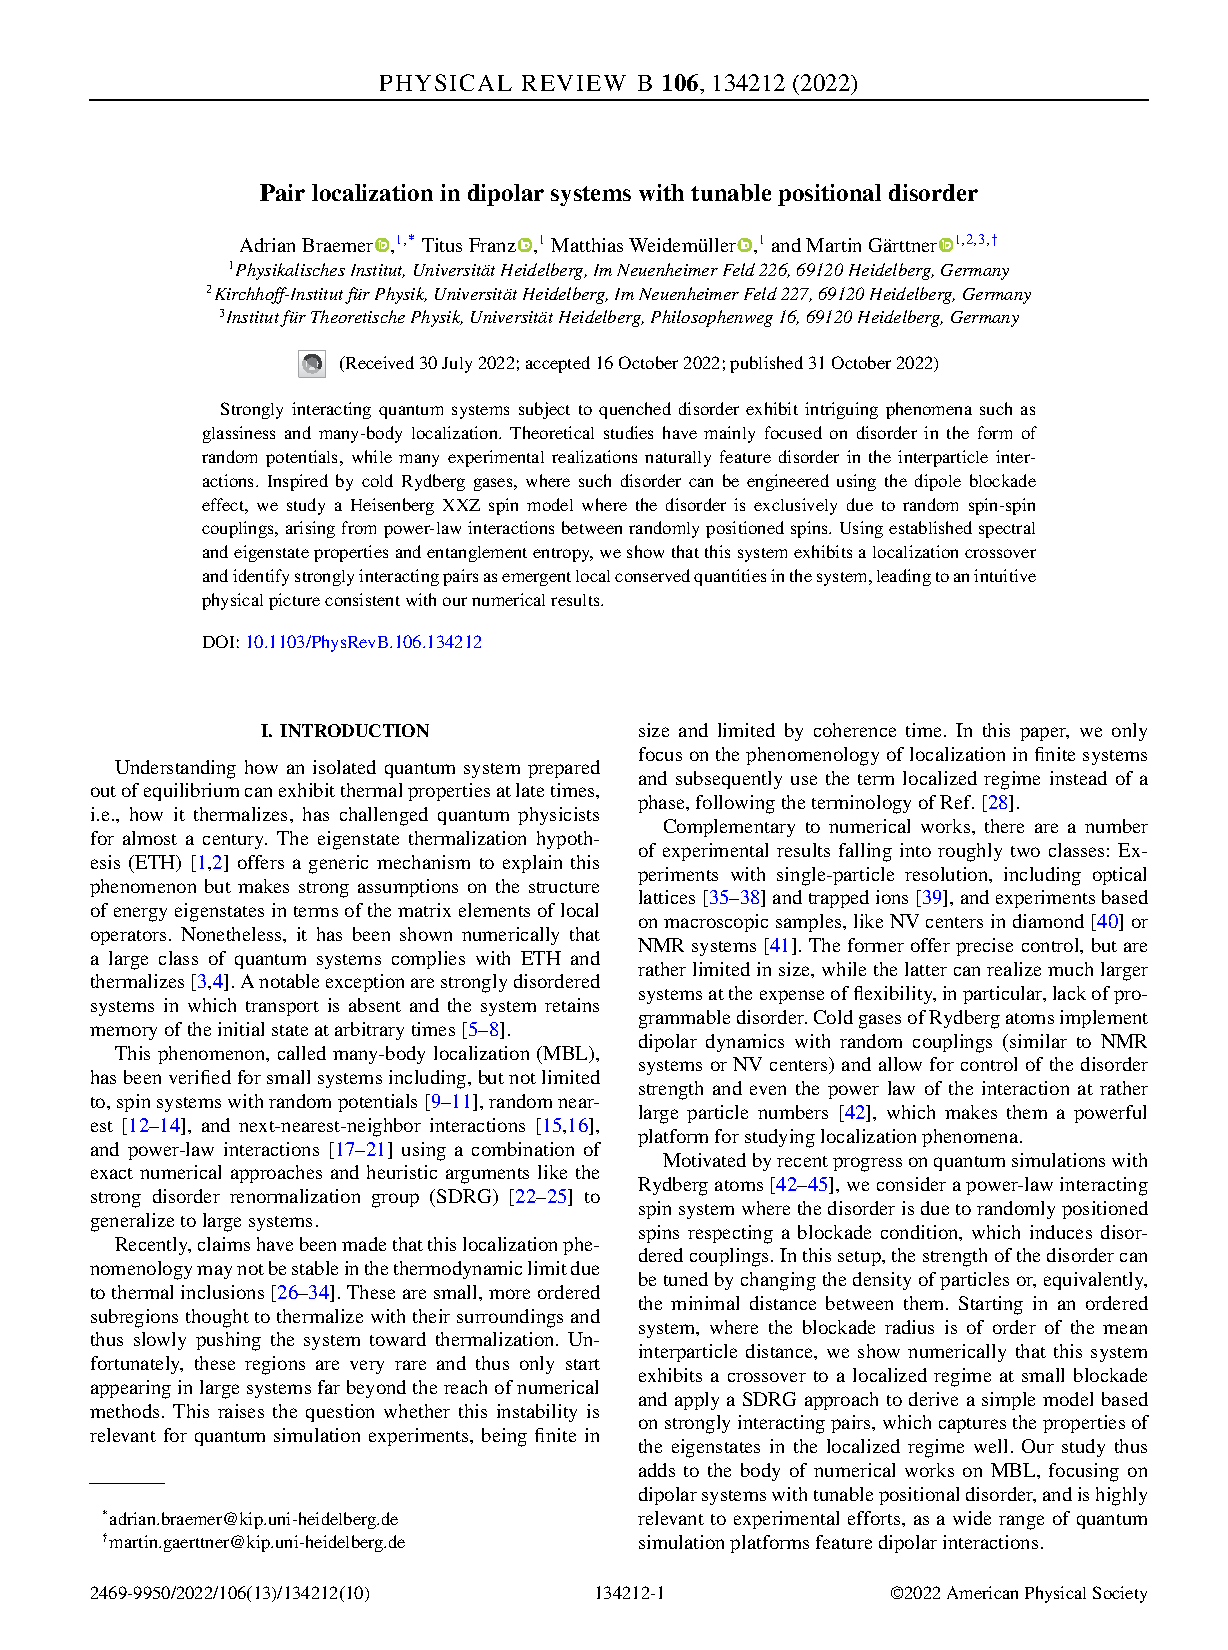
\includepdf[pages=-]{pub-Braemer2022-Pairlocalization}

\chapter{Efficient time evolution of pair localized systems}\label{ch:cTWA-paper}

After having found an analytical approximation applicable at strong disorder in the preceding chapter, here we show how to utilize this knowledge to achieve an efficient numerical computation of the dynamics. The key idea is to employ the cluster truncated Wigner approximation~\cite{wurtzClusterTruncatedWigner2018}, which is a semiclassical simulation method that solves the dynamics of only small clusters of spins exactly and treats interactions among clusters on a mean-field level. By using the pairing procedure of Chapter~\ref{ch:pair-localization-transition} to define the clusters, we find that our method is highly accurate not only at strong disorder and short-range interactions but also in regimes of comparatively weak disorder and long-range interactions. 
Thus, our method represents a numerically efficient scheme to compute arbitrary dynamical quantities in these kinds of spatially disordered spin systems.

% In addition, we generalize the cluster truncated Wigner approximation slightly to use a discrete phase-space sampling, which offers a minor boost in performance compared to continuous sampling and simplifies the implementation slightly since clusters of single spins no longer represent a special case. 
%TODO also mention the sampling? Not really important in the context of this work though
\newpage
\pdfbookmark[2]{Publication}{cTWA-paper}
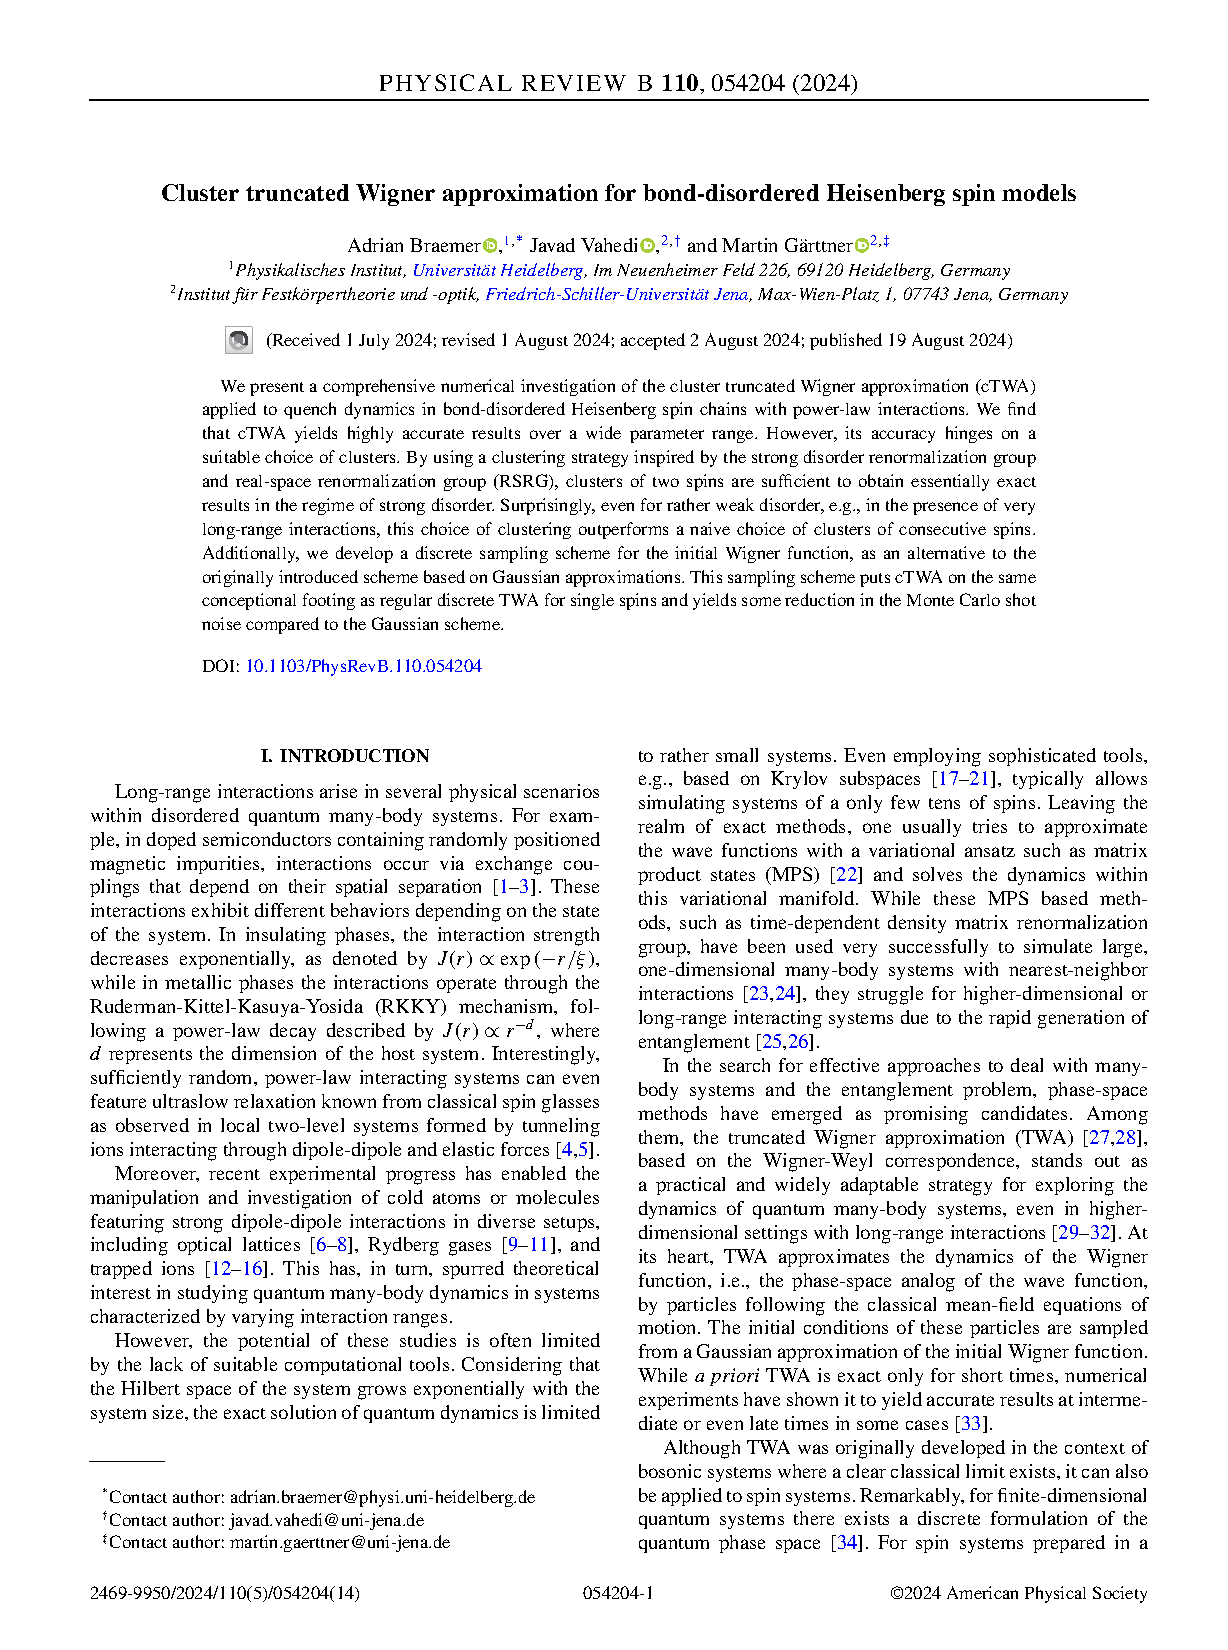
\includepdf[pages=-]{pub-Braemer2024-cTWA}

\chapter{Evidence of pair localization in the dynamics of Rydberg spins}\label{ch:experimental-pairs}

In this chapter, we apply the previously derived effective model of pairs to model and interpret experimental results from a Rydberg-based quantum simulator. While the experiment is limited to global control and readout, we make great use of its ability to implement models with different anisotropy and various density (which translates to disorder strength).

We find the pair model to yield  an excellent agreement with the observed behavior explaining both the relaxation dynamics and rescaling thereof~\cite{franzObservationAnisotropyindependentMagnetization2024} as well as the dependence of the steady state magnetization on the strength of the transverse field~\cite{franzEmergentPairLocalization2022}.


\section{Anisotropy-independent relaxation dynamics}\label{sec:universal-dynamics}
In this paper, we utilize the ability of the Rydberg quantum simulator to implement XX, XXZ and Ising models to measure the relaxation of the $x$-magnetization when starting from a fully magnetized state. For disordered Ising models prior work has shown the relaxation to follow a stretched exponential form well-known from spin glasses~\cite{breyStretchedExponentialDecay1993,signolesGlassyDynamicsDisordered2021,schultzenGlassyQuantumDynamics2022,schultzenSemiclassicalSimulationsPredict2022}. It has been conjectured that this type of slow, hierarchical relaxation is a common feature of strongly disordered quantum systems~\cite{haldarSlowDynamicsKohlrausch2023}.

Indeed we find that for all three models the relaxation curves are fitted well by stretched exponentials. Moreover, we also find a scaling law for the characteristic decay time scale which hints at a common origin of the relaxation. This mechanism is explained by the pair model, which yields that for all three models the relaxation is caused essentially by oscillations of the magnetization of pairs. Since each pair has a different oscillation frequency these individual oscillations dephase and thus cause the total magnetization to decay. From the parameter dependence of these pair oscillations, we recover the characteristic timescale for the global magnetization's decay. Thus demonstrating an effective pair localization at least over experimentally relevant timescales.

\newpage
\pdfbookmark[3]{Publication}{universal-dynamics-paper}
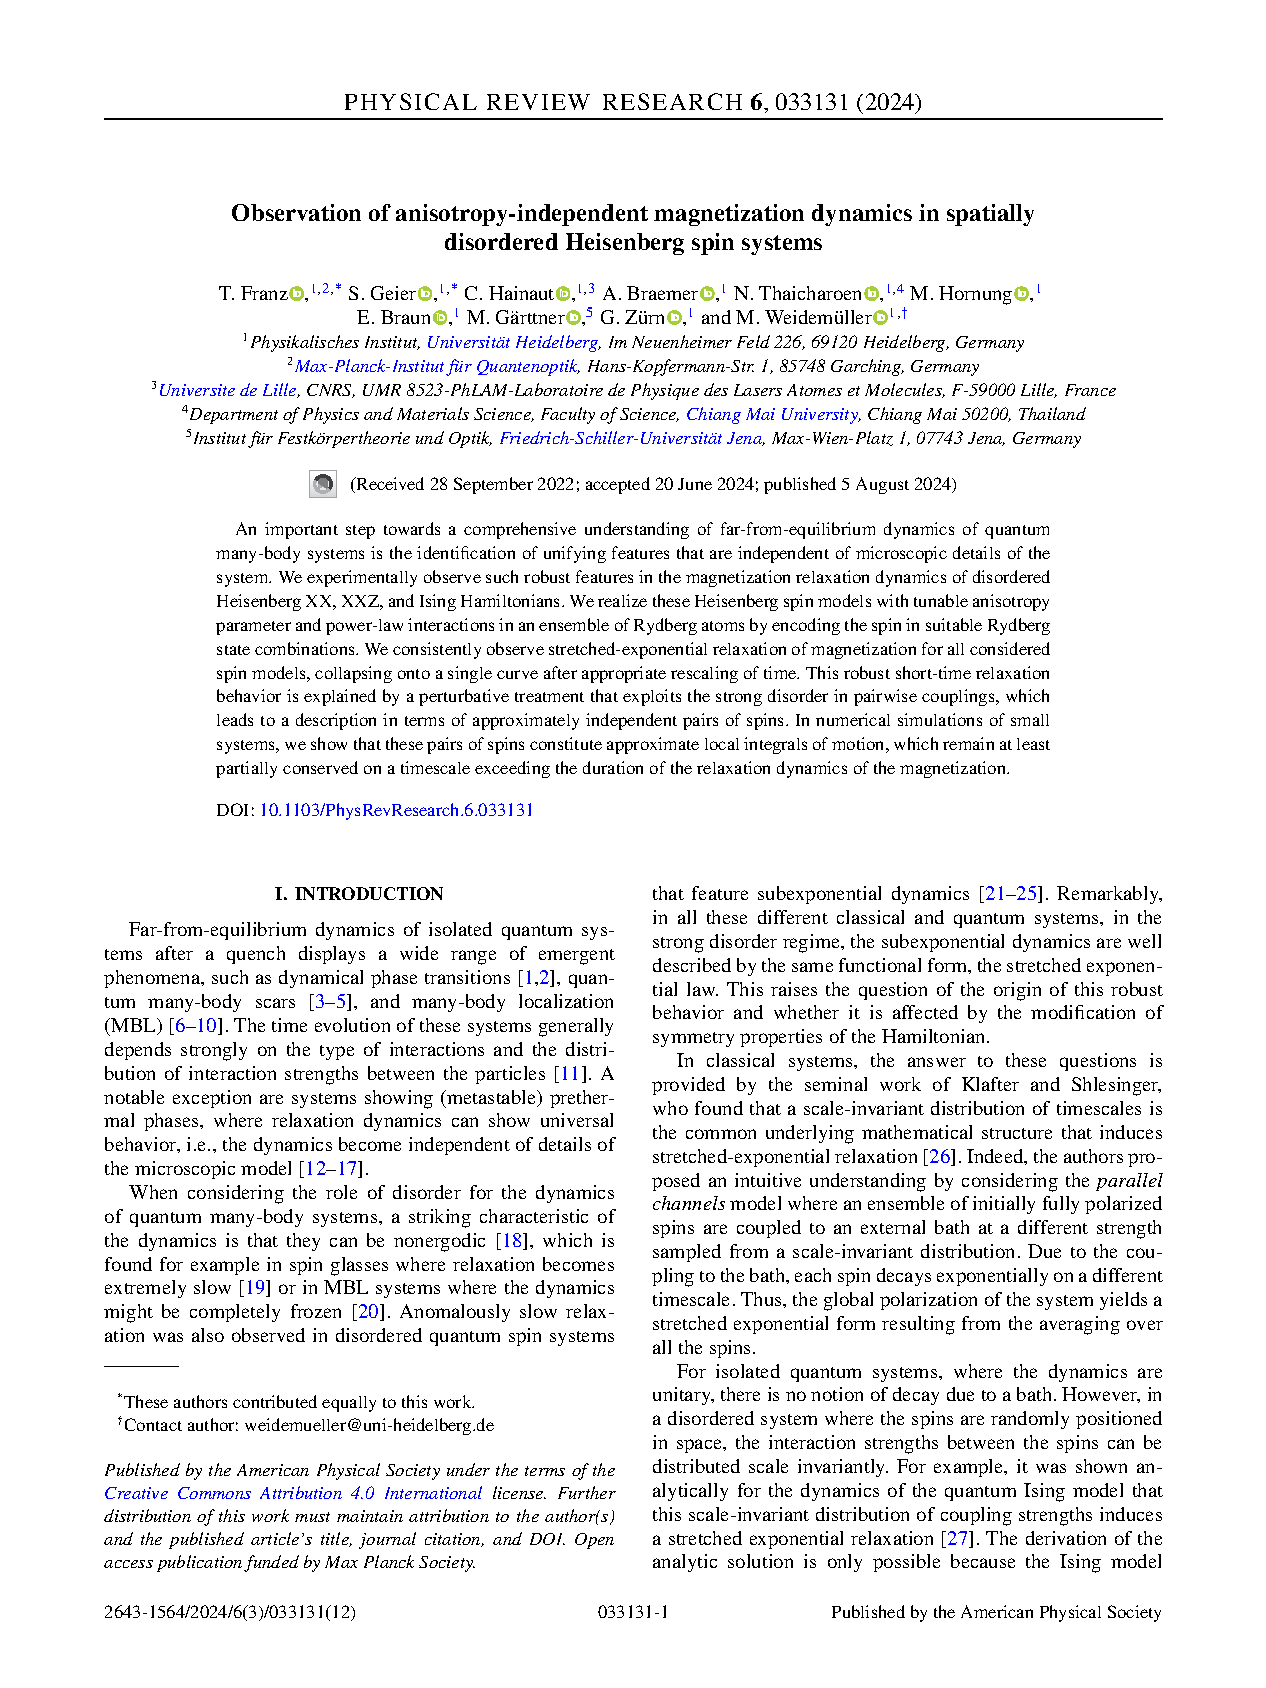
\includepdf[pages=-]{pub-Franz2023-UniversalDynamics}

\section{Emergent pair localization}
Another way of validating the pair model is the comparison of the same system subject different disorder strength. This can be realized in a Rydberg based quantum simulator by tuning the systems density as explained in the background chapter. %TODO reference

In the work below~\cite{franzEmergentPairLocalization2022}, we again use the $x$-magnetization as observable and track its steady-state value with respect to an external magnetic field aligned in $x$-direction as well. We find a clear qualitative difference at weak external field where the strongly disordered system responds much stronger to the field, i.e. the steady-state magnetization grows very fast with increasing field strength. This leads to a sharp cusp-like curve, which we show to be incompatible with a thermal state. However, we find that a pair-based effective model reproduces this feature and can also match the full measurement data closely.
In contrast, for weak disorder, i.e. high density, the behavior of the steady-state magnetization is much different. At weak field, the curve is very round which is reproduced nicely by assuming a thermal state.

Thus, this experiment provides direct evidence for a pair localization transition at least at experimentally relevant timescales. However, it is possible that this is a prethermal regime only and that this signature vanishes at much later times. Testing for this experimentally will of course be very hard if not impossible at all depending on the timescale this final relaxation occurs.

Subsequently in \autoref{sec:cusp-round-sharp}, we present an alternative to the mean-field model in \cite{franzEmergentPairLocalization2022}. This conceptually simpler model allows for analytical computation of both the thermal and pair localized magnetization curves. While this model is not as quantitative as the mean-field model contained in the publication, it nonetheless reproduces the curves qualitatively and highlights the physical origin of the behavior at weak field more directly.

\newpage
\pdfbookmark[3]{Publication}{cusp-paper}
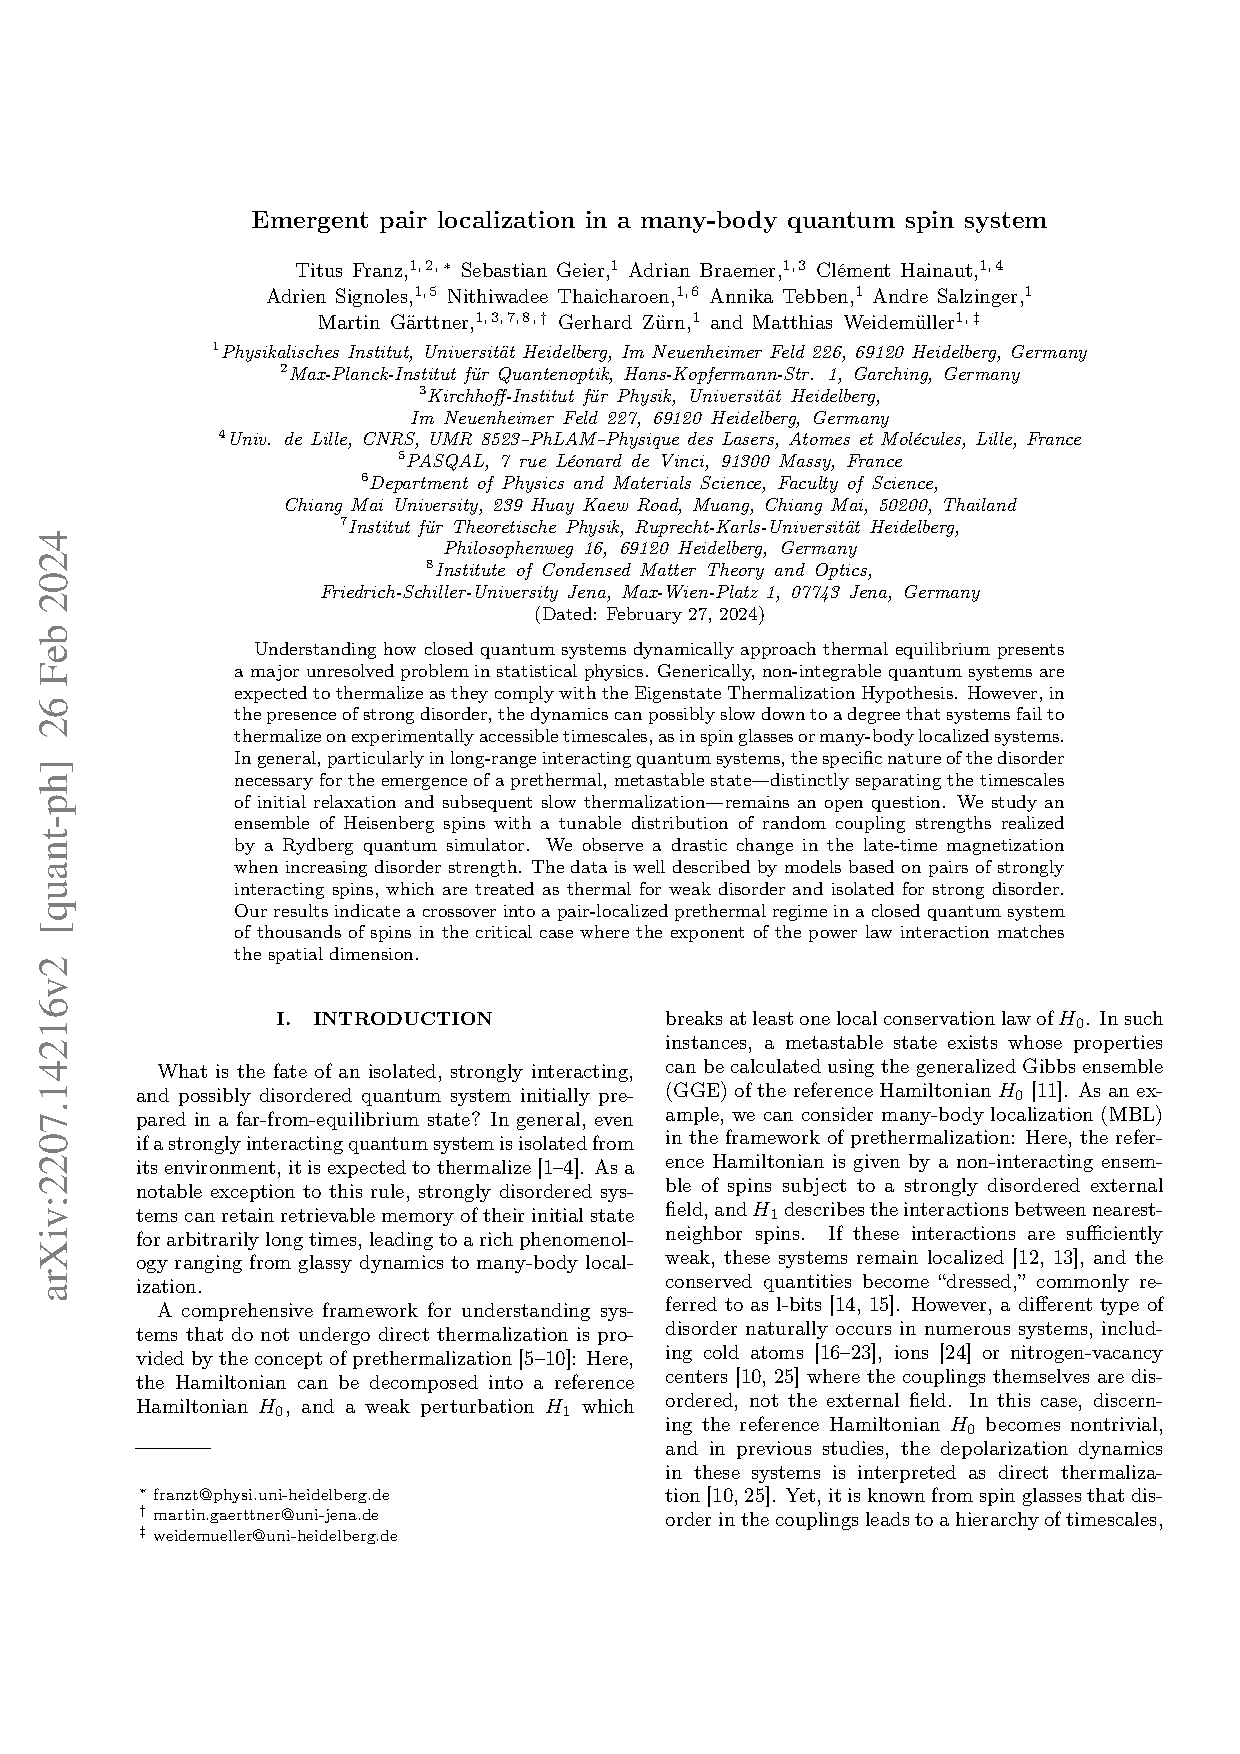
\includepdf[pages=-]{pub-Franz2022-Cusp}

\subsection{Simple physical picture}\label{sec:cusp-round-sharp}
To derive the qualitative behavior of the steady-state magnetization $\braket[1]{M(\Omega)}$ with respect to external field $\Omega$, we use a simple two-component model where each spin is either fully polarized or fully demagnetized. We assume that a spin's final state depends solely on the ratio of the strongest coupling $J$ towards another spin and the strength of the external field $\Omega$. If the field dominates, i.e. $|\Omega| > J$, the spin stays polarized as it is locked by the field. Conversely, if the coupling dominates, i.e. $|\Omega| < J$, then the interactions lead to depolarization and the spin loses its magnetization. Thus in this simplified model, the only quantity determining the steady-state magnetization is the distribution of relevant couplings $P(J)$:
\begin{equation}\label{eq:Cusp-simple-model-magnetization}
	\braket[1]{M(\Omega)} = \frac{1}{2}\int_0^{|\Omega|}\!\mathrm{d}J P(J)
\end{equation}

%TODO rephrase and use P_NN(J) as well
In the regime of weak disorder, it only natural to assume that the strongest relevant coupling for a spin is given by the coupling to its nearest neighbor. In contrast for strong disorder where we assume the pair model to describe the dynamics, the nearest neighbor coupling usually is not the relevant coupling! Instead, we need to consider the distribution of pair couplings $P_{pair}(J)$, i.e. the distribution of couplings that are shared by spins of the same pair.

To compute these coupling distributions analytically, we go to the limit of vanishing blockade radius, i.e. $r_b\rightarrow 0$, and assume that spins are distributed randomly with uniform density $\rho$ in $d$ dimensional space. Fixing some spin, this gives us for the number of spins in spherical shell of size $r$ and width $\mathrm{d}r$
\begin{equation}\label{eq:uniform-spin-distribution}
	w_u(r)\mathrm{d}r = d \rho \Omega_d r^{d-1}\mathrm{d}r = d\lambda (\lambda r)^{d-1}\mathrm{d}r
\end{equation}
where $\Omega_d = \frac{\pi^{d/2}}{\Gamma(n/2+1)}$ is the volume of a $d$-dimensional unit sphere and $\lambda^d = \rho \Omega_d$ is akin to the inverse mean distance between spins. We use this setup to compute both the distribution of nearest neighbor coupling $P_{NN}(J)$ and the distribution of pair couplings $P_{pair}(J)$ in the following sections.

\subsubsection{Nearest-neighbor coupling distribution $P_{NN}(J)$}

The distribution of the nearest neighbor couplings can be found using a simple ansatz~\cite{chandrasekharStochasticProblemsPhysics1943}. Consider some fixed spin and the density of spin $w(r)$ at distance $r$. Then the probability $P_{NN}(r)$ of finding the nearest neighbor of that fixed spin at distance $r$ should be proportional to both the probability of having a spin in that distance and the probability of having no closer neighbor. This gives us the following integral-equation 
\begin{align}\label{eq:nn-integral-eq}
	P_{NN}(r) = w(r)*\left(1-\int_0^r \mathrm{d}r' P_{NN}(r')\right)
\end{align}
which can be solved straight-forwardly by noting that it has the form $f' = -w f$ and using separation of variables. The solution reads:

\begin{equation}\label{eq:nn-distribution}
	P_{NN}(r) = w(r)\exp\left(-\int_0^r \!\mathrm{d}r' w(r')\right)\quad.
\end{equation}

Plugging in the distance distribution for uniform spin density $w_u(r)$ (cf. \autoref{eq:uniform-spin-distribution}) gives us a so-called Weibull distribution:

\begin{align}\label{eq:weibull-distribution}
	P_{NN}(r) = d \lambda^d r^{d-1} \exp(- \lambda^d r^d)
\end{align}

Finally, changing variables\footnote{Note, the change of variables also needs to transform the measure, i.e. we transform $P(r)\mathrm{d}r \!\rightarrow\! P(J)\mathrm{d}J$} from distance $r$ to coupling $J=r^{-\alpha}$ yields the sought-after distribution of nearest-neighbor couplings
%
%\begin{align}
%	r &= J^{-\frac{1}{\alpha}}\\
%	\mathrm{d}r &= \frac{-1}{\alpha}J^{-\frac{1}{\alpha}-1}\mathrm{d}J
%\end{align}
%
%The sign of the Jacobi-Determinant is to be neglect and we obtain:
%
\begin{equation}\label{eq:P-NN-J}
	P_{NN}(J) = \beta\lambda^d J^{-\beta-1} \exp\left(-\lambda^d J^{-\beta}\right)
\end{equation}
where $\beta=\frac{d}{\alpha}$.

\subsubsection{Distribution of pair couplings $P_{pair}(J)$}
%TODO clear up difference pair <-> NN?
We can derive the distribution of pair lengths in a similar fashion to \autoref{eq:nn-integral-eq}. The key insight about the difference between a nearest neighbor and the partner of a pair in the RSRG sense is that the two partners of the pair are in some sense each other's partner. In contrast the "nearest neighbor" property does not need to be reflexive. Denoting the pair coupling distribution as $P_{pair}(J)$, we write down the respective integral equation, which is very similar to \autoref{eq:nn-integral-eq}, except that the second factor gets squared because \emph{both spins} may not be part of a smaller pair:

\begin{align}\label{eq:pair-integral-eq}
	P_{pair}(r) = w(r)*\left(1-\int_0^r \mathrm{d}r' P_{pair}(r')\right)^2
\end{align}

%We can solve this equation rather easily by separation of variables (easy once you know what to do that is...):
%
%\begin{align}
%	w_P(r) = w(r)*\left(1-\int_0^r \mathrm{d}r' w_P(r')\right)^2\\
%	\Leftrightarrow \int_0^R \mathrm{d}r \frac{w_P(r)}{\left(1-\int_0^r \mathrm{d}r' w_P(r')\right)^2} = \int_0^R \mathrm{d}r w(r)\\
%	\Leftrightarrow \frac{1}{1-\int_0^R \mathrm{d}r' w_P(r')} - 1 = \int_0^R \mathrm{d}r w(r)\\
%	\Leftrightarrow \int_0^R \mathrm{d}r' w_P(r') = 1- \frac{1}{1 + \int_0^R \mathrm{d}rw(r)}\\
%	\Leftrightarrow w_P(R) = \frac{w(R)}{\left(1 + \int_0^R \mathrm{d}rw(r)\right)^2}\\
%	\Rightarrow w_P(r) = \frac{d\mathrm{vol}_d(1)r^{d-1}}{\left(1 + \mathrm{vol}_d(1)r^d\right)^2} = \frac{d}{\lambda} \frac{\left(\frac{r}{\lambda}\right)^{d-1}}{\left( 1+\left(\frac{r}{\lambda}\right)^d\right)^2}
%\end{align}

This equation can be solved in the same way as \autoref{eq:nn-integral-eq} and yields
\footnote{\autoref{eq:pair-distribution} was derived by a different method for $d=3$ by former Master student Péter Kaposvári in his Master thesis~\cite{peterMasterThesis}.}:

\begin{align}\label{eq:pair-distribution}
	P_{pair}(r) = \frac{w(r)}{\left(1+\int_0^r\!\mathrm{d}r' w(r')\right)^2}
\end{align}

Employing the distance distribution for uniform spin density $w_u(r)$ (cf. \autoref{eq:uniform-spin-distribution}) again gives us that the pair distances follow a \emph{log-logistic distribution} for spins of uniform density:

\begin{equation}\label{eq:log-logistic-distribution}
	P_{pair}(r) = \frac{d\lambda^d r^{d-1}}{\left(1 + \lambda^d r^d\right)^2 }
\end{equation}

Changing to distance $r$ to coupling $J=r^{-\alpha}$ yields:

\begin{equation}\label{eq:P-pair-J}
	P_{pair}(J) = \frac{\beta\lambda^d J^{-\beta-1}}{\left(1+\lambda^{d}J^{-\beta}\right)^2}
\end{equation}

\subsubsection{Analytical steady-state magnetization}

\begin{figure}[htb]
	\centering
%	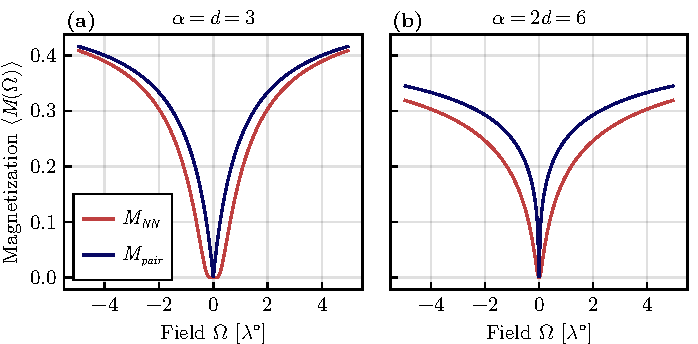
\includegraphics{part1/analytical_cusp}
	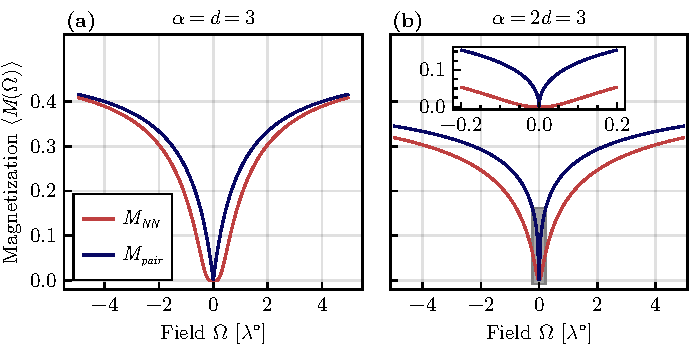
\includegraphics{part1/analytical_cusp_inset}
	\caption{Steady-state magnetization curves of the simple two-component model using the same color scheme as Fig.~2 (d) and (e) of \cite{franzEmergentPairLocalization2022}. Parameters, $\alpha$ and $d$ correspond to (a) Fig.~2 (b) Fig.~4.
	The inset show a zoom around $\Omega=0$ to highlight the qualitative difference between the curves.
	% TODO
	}
	\label{fig:analytical-cusp}
\end{figure}

Having derived both the distribution of nearest-neighbor coupling $P_{NN}(J)$ (cf. \autoref{eq:P-NN-J}) and pair coupling distribution $P_{pair}(J)$ (cf. \autoref{eq:P-pair-J}), we can compute the steady-state magnetization of our simple model by using \autoref{eq:Cusp-simple-model-magnetization}:
\begin{align}
	M_{NN}(\Omega) &= \frac{1}{2}\int_0^{|\Omega|}\!\mathrm{d}J\ P_{NN}(J) = \frac{1}{2}\exp(-\lambda^d |\Omega|^{-\beta})\\
	M_{pair}(\Omega) &= \frac{1}{2}\int_0^{|\Omega|}\!\mathrm{d}J\ P_{pair}(J) = \frac{1}{2+2\lambda^{d}|\Omega|^{-\beta}}
\end{align}

The resulting curves, shown in \autoref{fig:analytical-cusp}, show the same qualitative features as their counterparts in \cite{franzEmergentPairLocalization2022}. Thus, this simple model gives us insight in the key mechanism behind the qualitative change of the steady-state magnetization behavior: At weak field $|\Omega|\ll 1$, the magnetization is determined by the weakest interactions $J<|\Omega|\ll 1$ which stem from long distances $r \gg 1$. For nearest neighbors, the distribution of distances is suppressed exponentially $\propto \exp(-r^d)$ (cf. \autoref{eq:weibull-distribution}), which creates the very smooth, round shape at weak field. Conversely, if the relevant lengths are given by the pairing procedure, the exponential suppression is weakened to an algebraic decay $\propto r^{-d-1}$. Intuitively, this is because while with increasing distance $r$ the number of potential partners increases, it also becomes less likely that they are still available. This competition then leads to a much slower decay of the relevant lengths.

\subsubsection{Discussion}

\begin{figure}[htb]
	\centering
	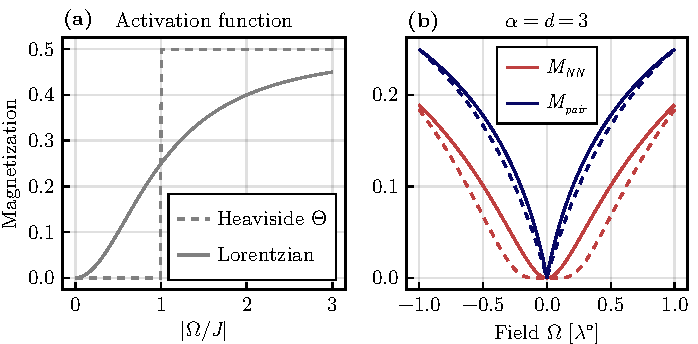
\includegraphics{part1/analytical_cusp_comparison_lorentz}
	\caption{Comparison of the two-component model (dashed lines) with another model where the constituents' magnetization is given by a Lorentzian (solid lines). (a) steady-state magnetization of the constituent. (b) predictions of both model for $\alpha=d=3$ [same parameters as \autoref{fig:analytical-cusp}(a)].
	}
	\label{fig:analytical-cusp-comparison-lorentz}
\end{figure}

The two-component model developed here is of course much simpler than the mean-field used in \cite{franzEmergentPairLocalization2022} but we argue that it captures the essential physics nonetheless. The two main conceptual differences are: The mean field model considers the magnetization response of pairs, which is a Lorentzian [cf. Eq.~(C3)], and additionally solves the equations self-consistently to capture the influence of a pairs magnetization on other pairs in the vicinity. The latter is responsible an the asymmetry of the ensemble's magnetization because the induced magnetization enhances (weakens) the effective magnetic field if external field and initial polarization are aligned (anti-aligned) to each other. This essentially introduces a small scaling factor for positive field for the field relative to negative values but does not change the qualitative behavior at weak field (cf. Fig.~5 of \cite{franzEmergentPairLocalization2022}). 

To check the effect of the Lorentzian magnetization function, we can generalize the two-component model slightly at the cost of it being no longer analytically solvable. We replace the idea of single spins that are either locked by the field or dominated by interaction by more general constituents that just follow some activation function, i.e. a function $m(\omega)$ that gives the resulting magnetization for a given ratio $\omega=\Omega/J$ of field strength $\Omega$ and relevant coupling $J$. Then the total steady-state magnetization reads

\begin{equation}\label{eq:generalized-two-component-model}
	\braket[1]{M(\Omega)} = \frac{1}{2}\int_0^{\infty}\!\mathrm{d}J P(J)m\left(\frac{\Omega}{J}\right)
\end{equation}
and the two-component model is recovered with $m(\omega)=\Theta(\omega - 1)$ where $\Theta$ denotes the Heaviside function. For a pair the magnetization follows a Lorentzian curve (cf. Eq.~(C3) of \cite{franzEmergentPairLocalization2022}), which in this notation is given by $m_L(\omega) = \frac{\omega^2}{1+\omega^2}$. As \autoref{fig:analytical-cusp-comparison-lorentz} shows, this does not alter the qualitative behavior at weak external field. Thus we conclude that the observed qualitative change of the steady-state magnetization stems from a fundamental change in character of the distribution of relevant couplings.

%Behavior around 0: Both non-analytic. $P_{NN}$ very round, all derivatives vanish. $P_{pair}$ non-analytic for $\beta\leq1$ i.e. $d \leq \alpha$.
%A few remarks:
%For $J\rightarrow 0$ this gives the limits:
%
%\begin{equation}
%	\lim_{J\rightarrow0} w_P(J) = \lim_{J\rightarrow0} \beta\lambda^{-d} J^{\beta-1} =\begin{cases}0 & d>\alpha\\ \beta\lambda^{-d} & d=\alpha\\ \infty & d<\alpha\end{cases}
%\end{equation}
%
%The Cusp thus acquires the form:
%
%\begin{equation}
%	\int_0^h\! \mathrm{d}J\ w_P(J) = \left. \frac{1}{1+\lambda^{d}J^{-\beta}}\right|_{0}^h = \frac{1}{1+\lambda^{d}h^{-\beta}}
%\end{equation}
%
%Note: For $\alpha > d$ this predicted cusp gets ultra sharp as the first derivative diverges at $0$!


%\begin{figure}[htb]
%	\centering
%	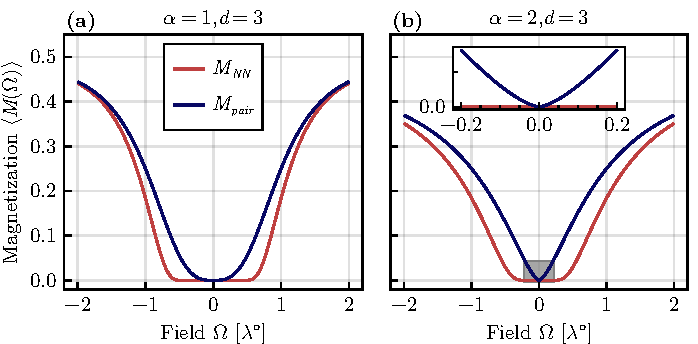
\includegraphics{part1/analytical_cusp_alpha_small}
%	\caption{Steady-state magnetization curves of the simple two-component model using the same color scheme as Fig.~2 (d) and (e) of \cite{franzEmergentPairLocalization2022}. Shown are two examples where $\alpha < d$.
%	}
%	\label{fig:analytical-cusp-alpha-small}
%\end{figure}



\chapter{Conclusion}
%Discussion&Outlook
% Summary
In Part 1 of this thesis, we studied long-range Heisenberg models subject to spatial disorder through the lens of many-body localization. We found that this type of disorder indeed leads to a MBL-like phase in small systems. In this regime, the dynamics is governed by the presence of quasi-local, conserved quantities, which are made up of pairs of strongly interacting spins. This result, when combined with cTWA, leads to a very efficient and accurate method to calculate the time evolution of observables. We showed two experimental signatures that we traced back to pairs being responsible for the dynamics and thus corroborated the model's applicability and predictive power in real-world scenarios.

% Conclusion for MBL
Of course an experiment can only offer data on finite times and finite system sizes and thus the big question of the existence of MBL in power-law systems~\cite{yaoManyBodyLocalizationDipolar2014,burinLocalizationRandomXY2015,burinManybodyDelocalizationStrongly2015,nandkishoreManyBodyLocalized2017} or even in general cannot be answered~\cite{deroeckStabilityInstabilityDelocalization2017,morningstarAvalanchesManybodyResonances2022,longPhenomenologyPrethermalManyBody2023,scoccoThermalizationPropagationFront2024}. However, we have shown that at least at experimentally accessible timescales MBL can be a very useful perspective on the dynamics even in $d=\alpha=3$. Since we have seen that the experiment can access both thermalizing regime and the localized regime (cf.~\cite{franzEmergentPairLocalization2022}), we can use it to locate the critical disorder strength and perform finite size scaling. Thus we can check experimentally both the presence of a \emph{prethermal} MBL regime (cf.~\cite{longPhenomenologyPrethermalManyBody2023}) and the drift of the crossover. Usually in models with on-site disorder, the crossover shows significant drift (see e.g.~\cite{luitzManybodyLocalizationEdge2015}) which is absent in the model studied here (see Fig.~5 of~\cite{braemerPairLocalizationDipolar2022}).  

% Other observables to learn more about the system, e.g. OTOCs
Due to experimental limitations, so far we only probed the global magnetization, which the pair model describes sufficiently accurate. In order to test its range of validity and shed more light on the properties of the system, it would be interesting to study more complex observables. A recent preprint found that already simple 2-point correlation functions like $\braket[1]{S_x^{(i)}S_x{(j)}}$ show significantly different late time behavior than predicted by the pair model~\cite{mukherjeeInfluenceDisorderedAnisotropic2024}. Accessing these in the current experiment could perhaps be realized through measurement of the variance of $\braket[1]{\sum_i S_x^{(i)}}$.
Another direction for future measurements are out-of-time-order correlators (OTOC) written as
\begin{equation}
	F(t) = \braket[1]{W^\dagger(t)V^\dagger W(t)V}.
\end{equation}
Here $W$ and $V$ are unitary operators that usually act locally. Then the OTOC provides information how much \emph{information} has been exchanged between the locations $W$ and $V$ act on~\cite{chenOutTimeOrder2017,swingleUnscramblingPhysicsOutoftimeorder2018,luitzEmergentLocalitySystems2019,xuScramblingDynamicsOutofTimeOrdered2024}. Thus OTOCs carry allow for a detailed diagnostic of the thermalization process (or lack thereof). This appears to be true even for OTOCS of global observables~\cite{lozano-negroGlobalOutTime2024}. However, measuring OTOCs is not an easy task since they generally require reversing the arrow of time for the system. While involved this can be achieved robustly by changing the states that encode the spin as demonstrated recently~\cite{geierTimereversalDipolarQuantum2024}. Another proposal based in Floquet Hamiltonian engineering is also in preparation~\cite{muellenbachOTOC}. 
These methods also open the wide field of echo protocols which find use e.g. in quantum enhanced sensing~\cite{davisApproachingHeisenbergLimit2016,linnemannQuantumEnhancedSensingBased2016,colomboTimereversalbasedQuantumMetrology2022}.
% OTOCs are a quite sensitive probe of the thermalization properties and can distinguish different forms of relaxation behavior

% improve RSRG by more RG
Addressing the question of the presence of MBL in systems with power-law interaction on the more theoretical side, one could extend RSRG-X to calculate higher order corrections of the pair model, which to our knowledge was not done so far. This extension owes to the fact that in power-law interacting systems the base Hamiltonian already contains interactions among spins that belong to different pairs. As such performing the iterative elimination that RSRG-X prescribes, implicitly assumes that the pair couplings also form a strong hierarchy, which is generally not true. Thus, one should eliminate all pairs simultaneously to obtain a new interactions among the pairs. Preliminary results indicate that when starting from a XX model ($\Delta=0$), this effective model of pairs assumes XXZ form, similar to a calculation by Burin~\cite{burinLocalizationRandomXY2015}. However, the simple interpretation of an ensemble of pairs is lost, as this effective model depends on the choice of the sectors of the pairs and thus for $N_p$ pairs there are $2^{N_p}$ different copies, similar to the problem with RSRG-t described in~\cite{monthusStrongDisorderRenormalization2018}. Interestingly, it could be that this picture can be reconciled with the iterative pairs criterion from~\cite{yaoManyBodyLocalizationDipolar2014} because the states described can be found in specific copies. This implies that there are eigenstates which entangle arbitrarily distant sites. Conversely, choosing an entangled pair state for each pair results in very weak effective hopping couplings and thus there are also states that are very to product states between pairs. It is hard to say what properties a typical choice would show. To summarize, it seems that considering effective pair-pair interactions gives rise to both states with long-range entanglement and localized states. This contradicts the idea of a global set of conserved quantities and thus would rule out MBL for these systems in a strict sense. Yet, it would also show that relaxation dynamics likely feature a strong hierarchy of timescales.
%When RSRG-X was developed in nearest neighbor interacting systems, perturbation theory was applied during the elimination to ensure that the spin chain stays connected. In other words, the spins adjacent to the eliminated pair experience a shared interaction mediated by fluctuations of the eliminated pair. 
% RSRG-X eliminates each coupling iteratively by freezing out the participating spins and thus makes the implicite assumption that each eliminated pair coupling is also much stronger than the next. 
%This allows for more detailed statements about the nature of information spreading: In thermalizing systems $F(t)$ should drop quickly to its minimal value dictated by symmetries and system size. Conversely, in localized systems A recent 

% effective time evolution and symmetry
\FIXME{Explain viewpoint of information: Initial state is permutation invariant, we can't even distinguish spins between shots, just measure global observable. Very little information extractable from a very complex computation.}
\marginline{A Lindbladian is defined by $\dot{\overline{\rho}} = \mathcal{L}_t[\overline{\rho}]$. If $\Lambda_t^{-1}$ exists, then $\mathcal{L}_t$ exists and reads: $\mathcal{L}_t = \dot{\Lambda}_t\circ\Lambda_t^{-1}$.}
A completely different route to understand the dynamics of disordered systems originates in the observation that a simple disorder-averaged expectation value can be seen as the expectation value of a single mixed state (overline denotes average w.r.t. disorder realization)
\begin{equation}
	\overline{\braket[3]{\psi(t)}{O}{\psi(t)}} = \Tr O \overline{\ket{\psi(t)}\bra{\psi(t)}} = \Tr O \overline{\rho}(t).
\end{equation}
The time evolution of this effective state $\overline{\rho}(t) = \Lambda_t[\rho_0]$ is governed by a dynamical map $\Lambda_t$, i.e. a super-operator mapping the initial density operator to the state at a later time. It is generally dissipative and non-markovian but under certain conditions can be mapped to a Lindblad description~\cite{kropfEffectiveDynamicsDisordered2016,gneitingIncoherentEnsembleDynamics2016,chenSimulatingOpenQuantum2018,gneitingDisorderdressedQuantumEvolution2020}. 
Although spatial symmetries are usually broken in each shot, the averaging leads to a restoration of these symmetries in the dynamical map $\Lambda_t$. This can potentially be quite powerful as spatially disordered systems oftentimes do not have a canonical order of the constituents and thus enjoy permutation invariance on average! Thus this approach has the potential to dispel the curse of dimensionality and might allow for the (numerical) simulation of large systems far beyond the reach of current methods. In a forthcoming publication~\cite{erpeldingSymmetries}, we explore this idea and show that one can indeed exploit the average symmetry to find a Taylor expansion of the effective Lindbladian for simple disorder distributions. While the numerical already look promising, more work is needed to generalize this approach to more realistic distributions such as the couplings arising from power-law interactions between randomly located sites.

%\section{Phase-diagram with integer distance statistics}



\part{Spatially inhomogeneous Floquet drive}\label{pt:floquet}
%************************************************
\chapter{Concepts: Periodically driven systems and time crystals}\label{ch:introduction-floquet}

The second, major, part of the thesis switches gear and focuses on the effects of spatial inhomogeneity in Floquet systems, i.e. systems that undergo periodic driving. While there has been a lot of attention already for Floquet systems with disorder in the interaction part of the cycle, most studies focus on the prototypical MBL model. Thus the consequences of pair localization or influence of disorder in the drive remain largely unstudied. Before, we explore these in the following chapters, first we give a brief overview of the relevant concepts from the field of Floquet systems. For a more in-depth review, we refer the interested reader to e.g.~\cite{eckardtColloquiumAtomicQuantum2017}. Subsequently, we also cover the basics of thermalization in Floquet systems (see e.g.~\cite{moriThermalizationPrethermalizationIsolated2018} for more context) and then briefly summarize the phenomenon of time crystals in particular~\cite{elseFloquetTimeCrystals2016,khemaniBriefHistoryTime2019,elseDiscreteTimeCrystals2020a}.

%review~\cite{eckardtColloquiumAtomicQuantum2017}

%time-dependent, periodic Hamiltonian -> at stroboscopic times can be modeled by time-independent Hamiltonian which is not unique but eigenenergies only defined up to mod $2pi/T$

\section{Introduction to Floquet systems}

Starting with the basics, a Floquet system is a system governed by a time-dependent Hamiltonian $H(t)$ with period $T$, i.e. 
\begin{equation}
	H(t) = H(T+t)\quad.
\end{equation}
The time evolution operator evolving the initial state to some time $t$ reads formally
\begin{equation}
	U(t) = \mathcal{T}\exp(-i\int_0^t\!\mathrm{d}t'H(t'))
\end{equation}
where $\mathcal{T}\exp$ is the time-ordered exponential.
Exploiting the periodicity, we can split the time evolution operator
\begin{align}
	U(t) &= \mathcal{T}\exp(-i\int_0^t\!\mathrm{d}t'H(t'))\\
	&= U(t-nT)\left[\mathcal{T}\exp(-i\int_0^T\!\mathrm{d}t'H(t'))\right]^n\\
	&= U(t-nT) (U_F)^n
\end{align}
into a $n$ application of an operator $U_F$, which advances the state a full cycle, and a \emph{micromotion} part $U(t-nT)$. So restricting the dynamics to \emph{stroboscopic} times where $t=nT$, we can understand the dynamics entirely by considering the time-independent operator
\begin{equation}
	U_F = \mathcal{T}\exp(-i\int_0^T\!\mathrm{d}t'H(t')) \equiv \exp(-iTH_F)
\end{equation}
where $H_F$ is a effective, time-independent Hamiltonian, called \emph{Floquet Hamiltonian}. There are some difficulties with this approach: First of all, $H_F$ is ill-defined because its eigenvalues are only defined $\mod 2\pi/T$. Owing to this fact, they are usually called \emph{quasienergies}. Secondly, $H_F$ is generally infeasible to calculate and might be grossly non-local.

In the following, we restrict the discussion to a typical setup where $H(t)$ consists of two parts: A part where the system undergoes dynamics according to its interactions $H_{int}$ and another part where the drive $H_{drive}$ is active and no other internal dynamics takes place:
\begin{align}
	H(t) &= \begin{cases}
		H_{int} & 0 \leq t < t_{int}\\
		H_{drive} & t_{int} \leq t < T=t_{int}+t_{d}
	\end{cases}\\
\Rightarrow\quad U_F &= \exp\left(-it_{d}H_{drive}\right)\exp\left(-it_{int}H_{int}\right) \label{eq:simple-floquet}
\end{align}
A simple way of approximating such a $H_F$ is through the \emph{Magnus expansion}, which is guaranteed to converge in the \emph{high frequency limit}, i.e. if $t_{int}\norm{H_{int}}+t_{d}\norm{H_{drive}} \ll \pi $~\cite{blanesMagnusExpansionIts2009}. In this simple case it amounts to applying the well-known Baker-Campbell-Hausdorff formula to Eq.~\ref{eq:simple-floquet}. The first few terms are given by:
\begin{align}
	H_F &= \sum_k H_F^{(k)}\\
	H_F^{(1)} &= \frac{1}{T}\left(t_{int} H_{int} + t_{d}H_{drive}\right)\\
	H_F^{(2)} &= \frac{t_{d}t_{int}}{2T} \left[H_{drive}, H_{int}\right]
\end{align}
Apart from being simple to calculated in most cases, the Magnus expansion is hermitian in every order and preserves the symmetries of the Floquet operator $U_F$. Additionally, for models featuring only two-body terms, the occuring operators only grow by a single site per order. This features make the Magnus expansion central to many approaches to Floquet systems.

In cases where one of the participating operators is not small, there exists another approach to approximate $H_F$ with similar properties which is based on a replica resummation trick~\cite{vajnaReplicaResummationBakerCampbellHausdorff2018}.

\section{Thermalization in Floquet systems}

The Floquet Hamiltonian $H_F$ allows to understand the dynamics of Floquet systems in the same terms as in closed quantum systems. So when viewed at stroboscopic times, the system thermalizes in accordance to $H_F$. Since this is not a true thermal equilibrium, because it is not stable for arbitrarily long times, this is usually called (Floquet) \emph{prethermalization}~\cite{moriThermalizationPrethermalizationIsolated2018}.

\FIXME{Visualize prethermalization}

When considering longer and longer times, higher and higher orders of the Magnus expansion become relevant leading to a slow drift of the equilibrium state. The general physical intuition is that the drive pumps energy into the system heating it up until it reaches a featureless infinite temperature state\cite{dalessioLongtimeBehaviorIsolated2014,bukovUniversalHighfrequencyBehavior2015}. It has been shown that the timescale this heating occurs on grows exponentially with the driving frequency $\omega\propto T^{-1}$~\cite{kuwaharaFloquetMagnusTheory2016,abaninRigorousTheoryManyBody2017}.

%Thermalization to $H_F$ similar to closed system.
%
%Usually driving deposits energy into the system causing heating towards an infinite temperature state \cite{dalessioLongtimeBehaviorIsolated2014,bukovUniversalHighfrequencyBehavior2015}.
%
%Prethermalization~\cite{moriThermalizationPrethermalizationIsolated2018}: In high frequency limit, there is a meta stable state given by Magnus expansion. When breakdown occurs, the systems continues heating. At high frequency, heating time grows exponentially

\section{Time crystals}

However, similar to closed systems, there are exceptions to this rule.
For example, it has been shown that a MBL interaction Hamiltonian can preserve the localization provided sufficiently fast driving~\cite{abaninTheoryManybodyLocalization2016,burauFateAlgebraicManybody2021,sierantStabilityManybodyLocalization2023}. 
A somewhat related but conceptually different mechanism is the phenomenon dubbed "time crystal"~\cite{vonkeyserlingkAbsoluteStabilitySpatiotemporal2016,elsePrethermalPhasesMatter2017}, where the (prethermal) equilibrium state breaks the discrete time-translation symmetry given by $U_F$~\cite{khemaniBriefHistoryTime2019,elseDiscreteTimeCrystals2020a}. A prototypical example~\cite{elseFloquetTimeCrystals2016,elseDiscreteTimeCrystals2020a} is a driven MBL system, where the LIOMs $\tau_z^{(i)}\approx\sigma_z^{(i)}$ are close to $\sigma_z$ and the drive approximately flips the system about it's $x$-axis, i.e.
\begin{align}
	H_{int} &= \sum_i h_i \tau_z^{(i)} + \sum_{ij} J_{ij}\tau_z^{(i)}\tau_z^{(j)}+\ldots\\
	H_{d}&=\exp(i(1-\epsilon)\pi\sum_i \sigma_x^{(i)}).
\end{align}
It is easy to see that at $\epsilon=0$, all the $\sigma_z^{(i)}$ are quasi-conserved in magnitude but switch their sign every period because $\sigma_x \sigma_z \sigma_x = -\tau_z$. Thus we can write
\begin{equation}
	U_F = X\exp(-i\sum_{ij} J_{ij}\tau_z^{(i)}\tau_z^{(j)} + \ldots )
\end{equation}
where $X\propto\prod_i \sigma_x$ and the exponential contains only the terms commuting with $X$. This means any $z$-basis state is (close to) an eigenstate of $U_F^2$ but not of $U_F$, which justifies the term \emph{time translation symmetry-breaking}~\cite{elseFloquetTimeCrystals2016}. The dynamics of such a state show a \emph{subharmonic response} because they oscillate with an integer multiple of the systems driving frequency.

Crucially, this phenomenon is stable to perturbations! Leaving the exactly soluble point at $\epsilon=0$, all of these features persist in a finite region of the parameter space. Thus time crystals truly represent an out-of-equilibrium phase of matter. Apart from the prototypical model above, there are many different scenarios where they can arise~\cite{khemaniBriefHistoryTime2019,elseDiscreteTimeCrystals2020a} and they have also been studied experimentally on a variety of platforms (e.g.~\cite{choiObservationDiscreteTimecrystalline2017,miTimeCrystallineEigenstateOrder2021,ippolitiManybodyPhysicsNISQ2021,randallManybodyLocalizedDiscrete2021}).
	



%************************************************
\chapter{Spatially-varying drive}\label{ch:metronome-spin}
% TODO better heading

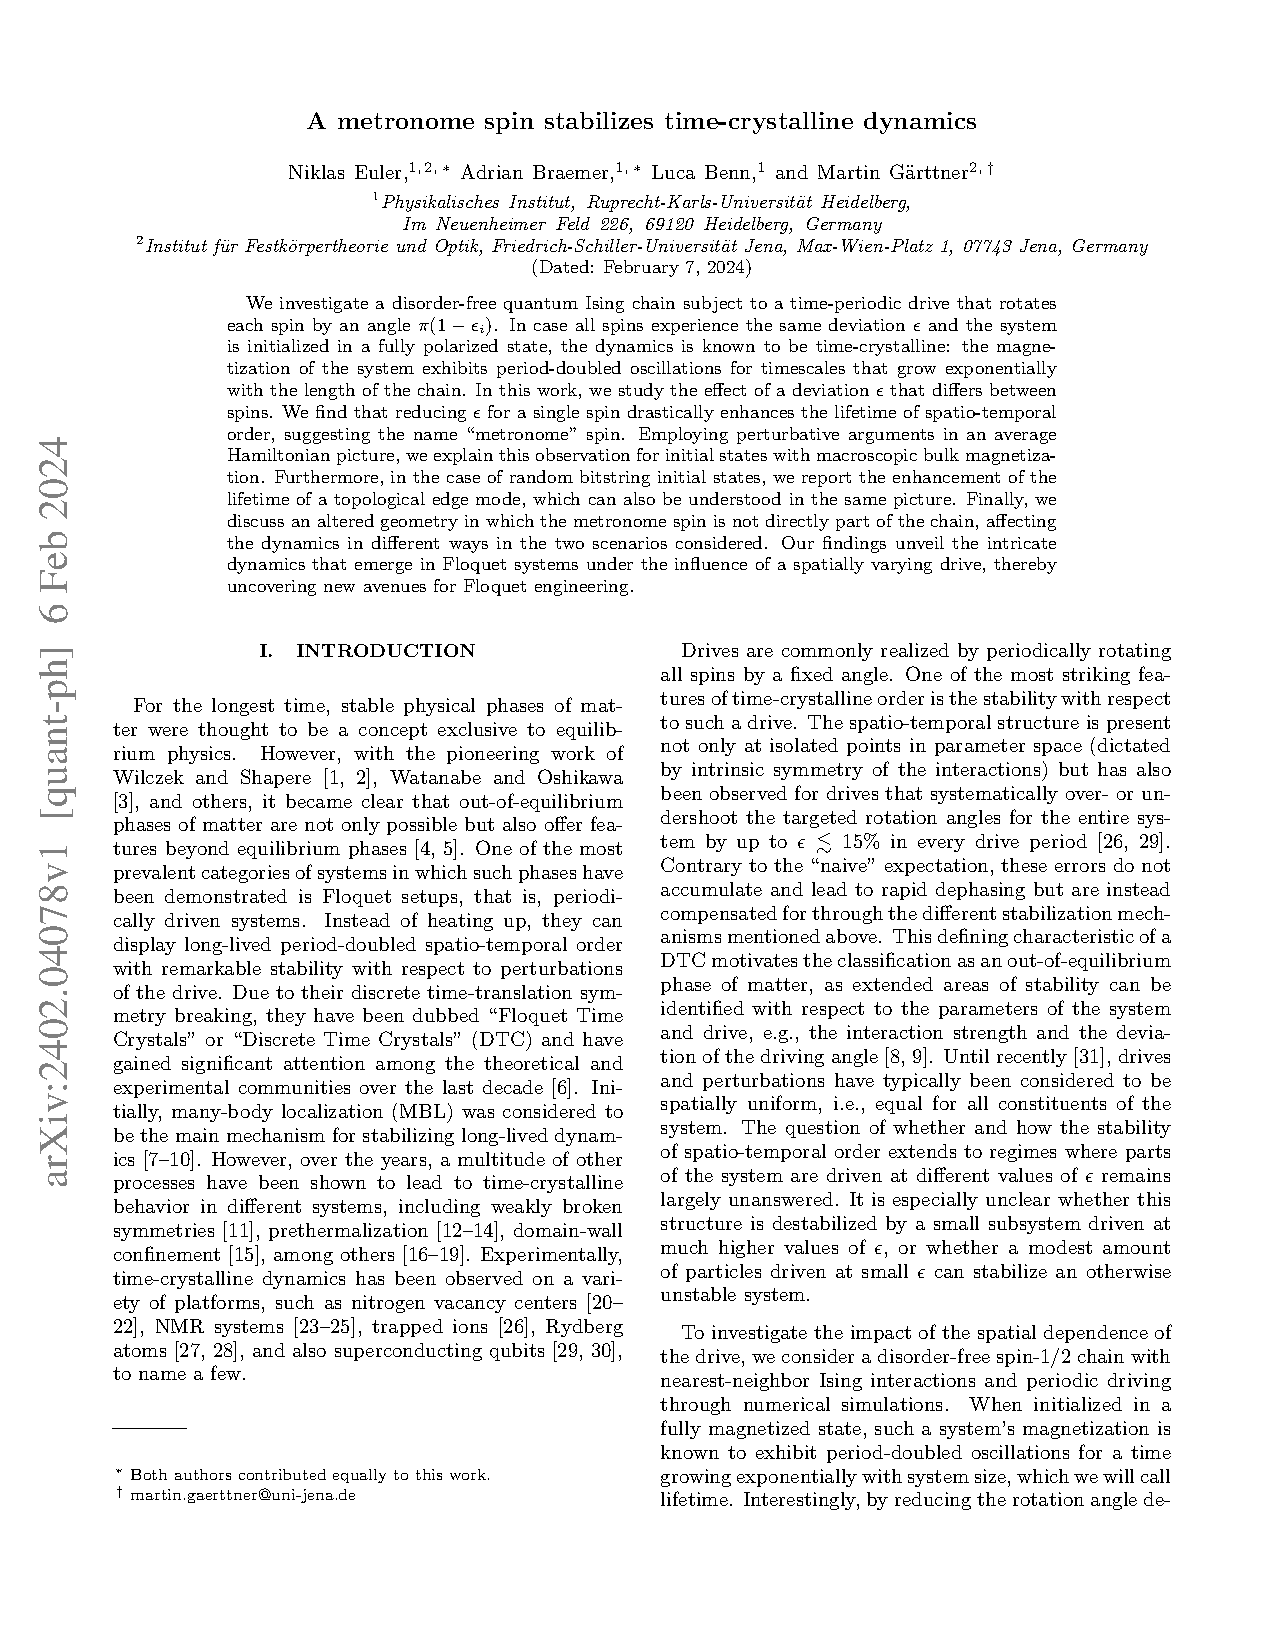
\includepdf[pages=-]{pub-Euler2024-MetronomeSpin}

%************************************************
\chapter{Outlook: Observation of a time crystal in the Rydberg Experiment?}
Novel stabilization mechanisms due to disorder?

\texttt{rydberg-pair-timecrystal.jl}
Replace interacting Hamiltonian with Pair model. Then dynamics are effectively average over pair  distribution. Each pair is not stable but has some lifetime depending on its interaction strength. Since distribution is very broad there is some phase-wrapping going on which leads to a slow decay. So pair model predicts not a stable time crystal but an anomalously slow decay (stretched exponential again?).

\chapter{Discussion}\label{ch:floquet-discussion}



\part{Summary}
%************************************************
%\chapter{Summary}
\label{pt:summary}
Two routes to non-thermalization (or to avoid thermalization at the usual short timescales) that both generate effectively conserved quantities in a subtle way.

% ********************************************************************
% Backmatter
%*******************************************************
% \appendix
%\renewcommand{\thechapter}{\alph{chapter}}
% \cleardoublepage
% \part{Appendix}
% \include{Chapters/Chapter0A}
%********************************************************************
% Other Stuff in the Back
%*******************************************************
\cleardoublepage%********************************************************************
% Bibliography
%*******************************************************
% work-around to have small caps also here in the headline
% https://tex.stackexchange.com/questions/188126/wrong-header-in-bibliography-classicthesis
% Thanks to Enrico Gregorio
\defbibheading{bibintoc}[\bibname]{%
  \phantomsection
  \manualmark
  \markboth{\spacedlowsmallcaps{#1}}{\spacedlowsmallcaps{#1}}%
  \addtocontents{toc}{\protect\vspace{\beforebibskip}}%
  \addcontentsline{toc}{chapter}{\tocEntry{#1}}%
  \chapter*{#1}%
}

%	\nocite{*}
\printbibliography[heading=bibintoc, resetnumbers=true, notkeyword=int]


\cleardoublepage%*******************************************************
% Acknowledgments
%*******************************************************
%\pdfbookmark[0]{Acknowledgments}{acknowledgments}
\phantomsection
\addcontentsline{toc}{chapter}{\tocEntry{Acknowledgments}}

\bigskip

\begingroup
\let\clearpage\relax
\let\cleardoublepage\relax
\let\cleardoublepage\relax
\chapter*{Acknowledgments}
% Martin 
First, I would like to thank my supervisor \emph{Martin Gärttner} for the great time I was allowed to spend within his group. Well, in the beginning when I started (for my master project), there did not exist much of a group but it steadily grew over time into its current size. Throughout the whole time, the atmosphere was always open, engaged and welcoming, which really is a reflection of your mentality. I really appreciate that I could seek your advice at any time and you always expressed excitement about my/our work. I will always remember my time spent with you and the group fondly.

% Matthias
Secondly, I want to thank my co-advisor \emph{Matthias Weidemüller} for the opportunity to work in so close collaboration with experiment. To me this was an ideal environment, where I could solve puzzles that actually have a counterpart in the real world. %I thoroughly enjoyed discussing physics with you and learned a lot in the process.

% reviewer Tilman Enss, committee Werner Aeschbach, Selim
I also thank \emph{Tilman Enss} for reviewing this thesis and the further members of my committee \emph{Selim Jochim} and \emph{Werner Aeschbach}.

% MBQD
Although briefly mentioned above, I want to express my appreciation for all of my colleagues and friends from the MBQD group. You all (and this includes past members in HD as well as the new crew in Jena) contributed to make this a enjoyable time - be it on our retreats or just during normal work.
I want to make a couple special shout-outs. Starting with \emph{Niklas Euler}, with whom I had the pleasure of sharing my office and from whom I learned the secrets of cooking with Seitan. Further, I want to shout-out my norse namesake \emph{Adrian \AA sen} with whom I went on an epic quest to see the northern lights and experience the darkness of the polar night. \emph{Javad Vahedi}, I really enjoyed our discussions about numerics and programming. And last but not least, \emph{Mirco Erpelding} who made the last year 112\% more enjoyable.

% Rydberg: Titus, Sebastian, Gerhard
Another big source of joy and motivation were the frequent discussions with the Rydberg team. Especially I want to thank \emph{Titus Franz} for easing my way into this project by sharing his knowledge about numerical simulations of the system. Towards the later part of my journey, \emph{Sebastian Geier} was a great partner for discussions as well. I want to express my gratitude to you both and also include \emph{Gerhard Zürn}. Thank you for your general excitement about the experiment, which made me always looking forward to our discussions, and for your patience in explaining more details about atomic physics or the experiment whenever my theorist's perspective was a bit too simplistic.

% Julia
For the numerical work, I exclusively used the Julia programming language~\cite{bezansonJuliaFreshApproach2017}, which has been a constant source of joy. It certainly was a cornerstone of this thesis together with many excellent libraries/tools that also deserve acknowledging: \texttt{DrWatson.jl}~\cite{datserisDrWatsonPerfectSidekick2020} (reproducible scientific projects), \texttt{Pluto.jl}~\cite{fonsvanderplasPlutoJl2024} (notebooks), \texttt{DifferentialEquations.jl}~\cite{rackauckas2017differentialequations}, \texttt{Makie.jl}~\cite{danischMakieJlFlexible2021} (plots) and \texttt{DataFrames.jl}~\cite{bouchet-valatDataframesJlFlexible2023}.

% Personal
Finally, I am very grateful for the continuous support of my friends and family. First and foremost, I want to express my heartfelt gratitude for my parents, \emph{Petra} and \emph{Achim}, who always encouraged my curiosity and supported me on every step of my way, and for also my sister \emph{Lucy}, who always believed in me and cheered me up in times of doubt.
Extra special love goes out to my wonderful partner \emph{Brini}, who always was there for me when I needed her. Especially in times where this thesis filled my mind you were very understanding, supportive and even drew those coffee cups for me (see \autoref{fig:classical-coffee} and \autoref{fig:localized-macciato}).
I am very grateful to have you in my life and I very much look forward to less stressful times to enjoy together with you.

\endgroup


\end{document}
% ********************************************************************
